%=======================================================================
%  Deep Reinforcement Learning based Admission Control and Network
%  Resource Allocation for Core Network Slicing
%
%  DRAFT SKELETON v2 -- restructured around the measured experimental
%  results (August 2026).
%
%  HOW TO USE THIS FILE
%  --------------------
%  Every paragraph slot has two parts:
%     1. A "% [Px] GUIDANCE:" comment block telling you exactly what the
%        paragraph must argue, which numbers to quote, and what to cite.
%     2. A draft paragraph in plain prose.
%  Rewrite the draft prose in your own voice; do not touch the LaTeX.
%  All tables, figures, equations, algorithms and cross-references are
%  already coded and populated with the real measured numbers.
%
%  !! READ THE "CLAIMS AUDIT" NOTE AT THE END OF THIS FILE BEFORE
%  !! SUBMITTING -- the previous abstract's headline numbers (47.5% and
%  !! 18%) are NOT supported by the experiments and have been replaced.
%=======================================================================
\documentclass[10pt,journal,comsoc]{IEEEtran}
\usepackage{amsmath,amsfonts}
\usepackage{algorithm}
\usepackage{array}
\usepackage{amssymb}
\usepackage{amsthm}
\usepackage[caption=false,font=normalsize,labelfont=sf,textfont=sf]{subfig}
\usepackage{textcomp}
\usepackage{stfloats}
\usepackage{url}
\usepackage{verbatim}
\usepackage{cite}
\usepackage{color}
\usepackage{multicol}
\usepackage{multirow}
\usepackage{epsfig}
\usepackage{epstopdf}
\usepackage{booktabs}
\usepackage{mathtools}
\newtheorem{definition}{Definition}
\usepackage{makecell}
\usepackage{algpseudocode}
\usepackage{tikz}
\usepackage{pgfplots}
\pgfplotsset{compat=1.17}
\usetikzlibrary{positioning,arrows.meta,fit,backgrounds}
\hyphenation{op-tical net-works semi-conduc-tor IEEE-Xplore}

% --- consistent colours for the two architectures / agents ------------
\definecolor{cUni}{RGB}{31,119,180}
\definecolor{cSep}{RGB}{255,127,14}
\definecolor{cGre}{RGB}{44,160,44}
\definecolor{cAco}{RGB}{148,103,189}
\definecolor{cRev}{RGB}{140,140,140}

\begin{document}

\title{Deep Reinforcement Learning based Admission Control and Network
Resource Allocation for Core Network Slicing: Feasibility Preservation
and the Conditional Value of Joint Routing}

\author{Pedro Amaral,~\IEEEmembership{Member,~IEEE}
\thanks{Pedro Amaral is with the Departamento de Engenharia Electrot\'ecnica e de Computadores, Faculdade de Ci\^encias e Tecnologia,
FCT/UNL, Universidade Nova de Lisboa, 2829-516 Caparica, Portugal; pfa@fct.unl.pt, and Instituto de Telecomunica\c{c}\~oes, 1049-001 Lisbon, Portugal}%
}

\markboth{IEEE Transactions on Network and Service Management,~Vol.~XX, No.~X, 2026}%
{Amaral: DRL Admission Control and Resource Allocation for Core Network Slicing}

\IEEEpubid{0000--0000/00\$00.00~\copyright~2026 IEEE}

\maketitle

%=======================================================================
\begin{abstract}
%-----------------------------------------------------------------------
% GUIDANCE (ABSTRACT): Rewrite in your voice, but keep this argument
% order and these numbers -- they are the measured ones.
%   1. Context: slicing in the IP/MPLS transport core; AC and RA are
%      coupled and NP-hard.
%   2. What we do: single DRL agent that jointly decides admit/reject and
%      which of K precomputed paths to use, on an explicit operator
%      topology, with a state built only from OSS/telemetry counters.
%   3. Two architectures: unified action space (one network) vs factored
%      (two Q-estimators, separate routing replay buffer).
%   4. Headline result (HONEST): +3.6% acceptance over a strong
%      bottleneck-aware greedy on the operator topology (5 seeds, paired
%      t=7.44), replicated at +3.8% on a structurally different topology.
%   5. THE MECHANISM (this is the paper's real contribution): the agent
%      learns to preserve future admissibility -- it keeps 54.9% vs
%      46.2% of arrivals feasible (+8.7pp). This is why it wins.
%   6. THE BOUNDARY CONDITION (second contribution): joint routing only
%      pays when the topology has routing headroom rho>0. rho=11.0% on
%      the operator topology (joint beats AC-only by +7.4%); rho=0.0% on
%      the Waxman topology (AC-only is then the better agent). rho is
%      computable a priori, without training.
%   7. Architecture: factored == unified at K=3, and is robust at K=8
%      where the unified agent degrades by 2.6%.
%   DO NOT re-introduce the old "47.5% more slices" / "18% more
%   fulfilled" claims. They are not supported. See CLAIMS AUDIT.
%-----------------------------------------------------------------------
Network slicing requires an operator to decide, for every incoming slice
request, whether to admit it and how to embed it on the physical
substrate. In the IP/MPLS transport core these two decisions are coupled:
admitting a slice consumes capacity that constrains future embeddings,
and the path chosen determines how much future capacity is consumed. We
formulate joint slice admission control and path-level resource
allocation for an operator core network as a Markov Decision Process
whose state is restricted to counters already exported by production
OSS/telemetry systems, and solve it with duelling deep Q-networks. Two
architectures are compared: a unified agent with a single joint action
space, and a factored agent with independent admission and routing
Q-estimators trained from separate replay buffers. On a real operator
topology the joint agent admits $3.6\%$ more slices than a strong
bottleneck-aware greedy policy (paired over five seeds, $t=7.44$), and
this advantage replicates at $3.8\%$ on a structurally different
synthetic topology. We show \emph{why}: the learned policy performs
non-myopic admissibility preservation, keeping $54.9\%$ of arrivals
routable against $46.2\%$ under greedy, a behaviour a myopic heuristic
cannot reproduce. We further show that the additional value of learning
routing jointly with admission is \emph{conditional} on the substrate
offering routing headroom, which we quantify with a statistic $\rho$
measurable without training: on the operator topology $\rho=11.0\%$ and
joint control outperforms admission-only control by $7.4\%$, whereas on
a topology with $\rho=0\%$ the admission-only agent is the stronger
design. Finally, the factored architecture matches the unified one for
small action spaces and is robust as the number of candidate paths
grows, where the unified agent degrades by $2.6\%$.
\end{abstract}
\IEEEpubidadjcol
\begin{IEEEkeywords}
Deep reinforcement learning, network slicing, admission control,
resource allocation, IP core networks, traffic routing, generalization.
\end{IEEEkeywords}

%=======================================================================
\section{Introduction}
%=======================================================================
%-----------------------------------------------------------------------
% [I-P1] GUIDANCE: Motivation. 5G/6G verticals with heterogeneous QoS
% share one physical substrate; slice management is the operator's
% control problem. Keep this close to your original opening paragraph --
% it was fine. Cite guan2021customized, bernardez2021machine.
%-----------------------------------------------------------------------
Next-generation networks must simultaneously support services whose
traffic profiles and quality-of-service requirements differ by orders of
magnitude. In the 5G and beyond service-oriented model, distinct
verticals coexist over a common physical infrastructure, which makes the
efficient management of network slices a central operational problem for
network operators~\cite{guan2021customized,bernardez2021machine}.

%-----------------------------------------------------------------------
% [I-P2] GUIDANCE: Name the two coupled sub-problems (admission control,
% resource allocation) and state the coupling explicitly, because the
% coupling is what this paper is about: admitting now consumes capacity
% that constrains later admissions, and the path chosen decides how much.
% This sentence sets up the whole paper.
%-----------------------------------------------------------------------
Two decisions sit at the core of slice management. Admission control
determines whether an arriving slice request can be accepted, while
resource allocation assigns substrate resources -- in a transport core,
a route and a bandwidth reservation -- to the slices that are admitted.
These decisions are not independent. Every admission consumes capacity
that will be unavailable to later requests, and the path selected for an
admitted slice determines precisely which links become scarce. A policy
that treats the two in isolation therefore optimises a distorted version
of the operator's actual problem.

%-----------------------------------------------------------------------
% [I-P3] GUIDANCE: Why exact optimisation fails -> motivates model-free
% DRL. Mention NP-hardness (forward reference to Sec III-B), the
% unavailability of accurate traffic/demand models, and the online
% sequential nature. Cite sutton2018reinforcement, luong2019applications.
%-----------------------------------------------------------------------
The joint problem is computationally intractable and, worse, poorly
specified: it inherits the NP-hardness of multicommodity flow with
admission control, and it must be solved online, under an arrival process
that operators cannot model accurately in advance. These two properties
together motivate a model-free approach. Deep Reinforcement
Learning~\cite{sutton2018reinforcement} learns a control policy directly
from interaction, without requiring an explicit model of the environment
dynamics, and has been applied successfully to a range of networking
optimisation problems~\cite{luong2019applications}.

%-----------------------------------------------------------------------
% [I-P4] GUIDANCE: The gap. Existing DRL slicing work is RAN-centric or,
% when it addresses the core, models it at aggregate level without
% path-level routing; VNE work is generic and architecturally heavy.
% Cite ssengonzi2022survey, saha2023deep, villota2022admission,
% wang2024fsac, xiong2024hrlacra, sulaiman2025datadriven.
% Also state the transport-network angle: IP/MPLS cores already carry
% backhaul/enterprise/Internet and must absorb slicing (10258168).
%-----------------------------------------------------------------------
Although DRL has been applied widely to network
slicing~\cite{ssengonzi2022survey}, the literature concentrates on the
radio access network and on service function chain orchestration, with
comparatively little attention to the transport
domain~\cite{saha2023deep}. Works that do target the 5G core generally
model it at an aggregate resource level and do not take path-level
routing decisions on an explicit
topology~\cite{villota2022admission,wang2024fsac,sulaiman2025datadriven},
while the closely related virtual network embedding literature targets
generic substrates with architecturally heavy hierarchical
policies~\cite{xiong2024hrlacra,wang2024flagvne}. This leaves the
operator IP/MPLS core -- which already carries backhaul, enterprise and
Internet services and must now absorb slice traffic
as well~\cite{10258168} -- largely unaddressed.

%-----------------------------------------------------------------------
% [I-P5] GUIDANCE: State what we actually did, and be explicit that the
% study is as much about WHEN the joint approach helps as about IT
% helping. This is the honest framing and it is also the more useful
% contribution. Say plainly that we evaluate on two topologies and two
% load regimes and report where the method does and does not win.
%-----------------------------------------------------------------------
In this work we formulate joint admission control and path-level resource
allocation for the operator IP core as a single Markov Decision Process,
restrict the state to counters that production OSS and telemetry systems
already export, and solve it with duelling deep Q-networks. Rather than
reporting a single aggregate improvement figure, we set out to establish
under what conditions the approach is worth deploying: we evaluate two
agent architectures on two structurally different topologies across two
load regimes, we identify the behavioural mechanism that produces the
gains, and we report the regimes in which the joint formulation offers no
benefit over a simpler admission-only design.

%-----------------------------------------------------------------------
% [I-P6] GUIDANCE: Contributions list. Keep the itemised form. The
% ordering is deliberate: mechanism first, boundary condition second,
% because those are the durable contributions; raw margin is third.
% Quote the numbers exactly as written below.
%-----------------------------------------------------------------------
The specific contributions of this work are the following:
\begin{itemize}
  \item \textbf{A deployable joint formulation.} An MDP for joint slice
  admission and path selection on an explicit IP/MPLS core with per-link
  capacity constraints, whose state uses only readily available
  telemetry counters, together with a low-dimensional per-path
  feasibility signal that makes the routing decision learnable without
  exposing privileged network state.
  \item \textbf{Identification and measurement of the mechanism.} We show
  that the learned policy's advantage over a strong greedy baseline comes
  from \emph{non-myopic admissibility preservation}: it declines
  admissible requests in order to keep the substrate routable, sustaining
  $54.9\%$ feasible arrivals against $46.2\%$ for greedy on the operator
  topology, and $53.3\%$ against $46.7\%$ on a second topology. This
  explains, rather than merely reports, the performance difference.
  \item \textbf{A boundary condition for joint routing, measurable a
  priori.} We define a routing-headroom statistic $\rho$ -- the fraction
  of arrivals that are admissible on some candidate path but not on the
  shortest one -- and show it predicts whether joint control beats
  admission-only control. With $\rho=11.0\%$ the joint agent wins by
  $7.4\%$; with $\rho=0\%$ the admission-only agent is superior. $\rho$
  requires no training to evaluate.
  \item \textbf{An architectural comparison with a scaling result.} A
  factored design with independent admission and routing Q-estimators and
  a dedicated routing replay buffer matches the unified design at $K=3$
  and remains stable at $K=8$, where the unified agent's accuracy
  degrades by $2.6\%$.
  \item \textbf{Honest characterisation of the operating envelope.} We
  report the load regime in which the advantage is largest and the
  regimes and interventions where it disappears, including a negative
  result for feasibility-based action masking.
\end{itemize}

%-----------------------------------------------------------------------
% [I-P7] GUIDANCE: Roadmap paragraph. Mechanical; keep short.
%-----------------------------------------------------------------------
The remainder of the paper is organised as follows.
Section~\ref{State_of_Art} reviews related work.
Section~\ref{model} presents the system model, the problem formulation
and its MDP encoding. Section~\ref{agents} describes the two agent
architectures. Section~\ref{expSetup} details the simulation framework
and experimental protocol. Section~\ref{results} reports results and
Section~\ref{discussion} discusses their implications and limitations.
Section~\ref{conclusion} concludes.

%=======================================================================
\section{State of the Art} \label{State_of_Art}
%=======================================================================
%-----------------------------------------------------------------------
% [S-P1] GUIDANCE: One framing sentence for the section, then the
% subsections. Keep your original taxonomy -- it was good -- but the
% closing positioning subsection must now be rewritten around the
% mechanism / boundary-condition framing rather than "we beat everyone".
%-----------------------------------------------------------------------
We organise the related literature by the scope of the control problem
addressed, and close by positioning this work with respect to each group.

\subsection{Surveys}
%-----------------------------------------------------------------------
% [S-P2] GUIDANCE: Unchanged from your draft; the three surveys and what
% each concludes. Keep it to three or four sentences.
%-----------------------------------------------------------------------
Several surveys map the application of DRL to network slicing.
A broad overview of DRL in 5G slicing and virtualisation is given
in~\cite{ssengonzi2022survey}, which finds that most contributions target
the radio and edge segments. The survey in~\cite{hurtado2022deep}
examines DRL for slice resource management and observes that admission
control and allocation are frequently decoupled and evaluated only in
simplified radio models. Slice scaling and placement via DRL are reviewed
in~\cite{saha2023deep}, again with a radio focus and without core network
constraints.

\subsection{Resource-Allocation-Only and Admission-Control-Only Solutions}
%-----------------------------------------------------------------------
% [S-P3] GUIDANCE: Merge your two original subsections here to save
% space; the point is simply that these works solve one half of the
% problem. RA-only: kim2019reinforcement, van2019optimal, abiko2020flexible.
% AC-only: sciancalepore2019rl, 10293471, 9771643, 10437226, Tao_2025.
% End with the sentence that our AC-only DQN baseline is precisely this
% class, which is why we include it as an ablation.
%-----------------------------------------------------------------------
A first group addresses only resource allocation within already admitted
slices. Deep Q-networks and duelling architectures have been used to
allocate bandwidth across radio slices~\cite{kim2019reinforcement}, for
real-time slicing in virtualised radio access
networks~\cite{van2019optimal}, and for flexible resource block
assignment under time-varying demand~\cite{abiko2020flexible}. A second
group addresses only admission control. A reinforcement learning slice
broker that admits or rejects bids to maximise operator revenue is
proposed in~\cite{sciancalepore2019rl}; deterministic policy gradient and
actor-critic formulations for admission in resilient 5G networks appear
in~\cite{10293471}; and several value-based algorithms are compared for
revenue-maximising admission in~\cite{9771643}, with further examples
in~\cite{10437226,Tao_2025}. This second class corresponds exactly to the
admission-only baseline we use as an ablation in
Section~\ref{results}, since it isolates the contribution of learning the
routing decision.

\subsection{Admission Control and Resource Allocation in 5G Cores}
%-----------------------------------------------------------------------
% [S-P4] GUIDANCE: villota2022admission (SARA/DSARA), wang2024fsac
% (digital twin, partial admission), and the NEW reference
% sulaiman2025datadriven (data-driven online AC+RA, 2025). The critical
% observation to make: all of them model the core as aggregate resource
% pools, so path-level routing never enters the action space -- which is
% exactly the decision whose value this paper measures.
%-----------------------------------------------------------------------
A growing body of work addresses admission and allocation jointly in the
5G core. SARA and DSARA process slice requests in time windows and
optimise provider revenue and resource utilisation with reinforcement
and deep reinforcement learning~\cite{villota2022admission}. A flexible
admission scheme learning a partial-admission policy inside a digital
twin of the core is proposed in~\cite{wang2024fsac}, enabling exploration
without disturbing production traffic. More recently, data-driven online
admission and allocation for 5G and beyond has been formulated with
explicit demand uncertainty~\cite{sulaiman2025datadriven}. These works
establish the relevance of learned admission policies for the core, but
they represent the substrate as aggregate resource pools per node or per
slice type. Path-level routing consequently never appears in the action
space, and the question of whether learning it jointly with admission is
worthwhile is left open.

\subsection{Joint Solutions and Virtual Network Embedding}
%-----------------------------------------------------------------------
% [S-P5] GUIDANCE: RAN-centric joint work (Rezazadeh2021ZerotouchCN,
% 9322237, 9953137, zhou2022learning); core work that leaves routing to a
% heuristic (li2023reinforcement); 9655323 which does routing but assumes
% slices are pre-admitted; and VNE (xiong2024hrlacra, and NEW
% wang2024flagvne which explicitly targets generalization across
% instances). Make the point that generalization across substrates is
% recognised as the open issue in VNE -- this motivates our two-topology
% evaluation.
%-----------------------------------------------------------------------
Joint formulations exist but differ in domain or in the placement of the
routing decision. Actor-critic methods have been applied to joint
admission and allocation in the radio access
network~\cite{Rezazadeh2021ZerotouchCN,9322237}, including multi-agent
designs with graph attention for topology
generalisation~\cite{9953137} and transfer learning across radio and
cache resources~\cite{zhou2022learning}; all optimise radio-specific
objectives. In the core, admission has been learned while resource
recycling is delegated to a heuristic~\cite{li2023reinforcement},
whereas multi-task learning with graph convolutional networks performs
slicing and routing but assumes requests are admitted a
priori~\cite{9655323}. In virtual network embedding, hierarchical
reinforcement learning has been used to combine admission and embedding
decisions~\cite{xiong2024hrlacra}, and recent work explicitly targets
generalisation across problem instances and substrate
sizes~\cite{wang2024flagvne}, confirming that transferability across
substrates -- not raw performance on a single graph -- is the open issue
in this family of problems. That observation directly motivates the
two-topology evaluation adopted here.

\subsection{Positioning of This Work}
%-----------------------------------------------------------------------
% [S-P6] GUIDANCE: Rewrite of your old positioning list. The key change:
% we no longer claim to beat everything. We claim (i) path-level routing
% in the action space on a real core, (ii) OSS-only state, (iii) we
% identify the mechanism, (iv) we give a measurable condition under which
% the joint approach is worth its extra complexity, (v) two topologies.
% Point (iv) is the novel one -- no prior work states when joint AC+RA is
% NOT worth deploying. Reference Table~\ref{tab:related_work_comparison}.
%-----------------------------------------------------------------------
Table~\ref{tab:related_work_comparison} summarises the comparison. Our
work differs in five respects. First, the routing decision is inside the
agent's action space and is taken over explicit paths on an operator
IP/MPLS topology with per-link capacity constraints, rather than over
aggregate resource pools. Second, the state is restricted to counters
available from existing OSS and telemetry, which keeps the policy
deployable. Third, we identify and measure the behavioural mechanism
responsible for the improvement instead of reporting only aggregate
gains. Fourth, and to our knowledge not addressed in prior work, we
provide a substrate statistic that predicts \emph{whether} the joint
formulation will outperform a simpler admission-only controller, and we
report a topology where it does not. Fifth, all conclusions are
evaluated on two structurally different topologies and two load regimes.

\begin{table*}[t]
\caption{Comparative overview of related work.}
\centering
\renewcommand{\arraystretch}{1.2}
\begin{tabular}{>{\raggedright\arraybackslash}m{1.8cm}
                >{\raggedright\arraybackslash}m{4.0cm}
                >{\raggedright\arraybackslash}m{2.7cm}
                >{\raggedright\arraybackslash}m{1.9cm}
                >{\raggedright\arraybackslash}m{5.4cm}}
\toprule
\textbf{Reference} & \textbf{Scope} & \textbf{DRL methodology} & \textbf{Scenario} & \textbf{Key differences vs.\ this work} \\
\midrule
\cite{Rezazadeh2021ZerotouchCN,9322237} & Joint admission \& resource allocation & Actor--critic (TD-DDPG) & RAN & Radio objectives; no path-level routing or per-slice bandwidth on a core topology \\
\cite{9953137} & Joint admission \& embedding & Multi-agent DRL + GAT & RAN/MEC & Tailored to RU/DU/CU functional split \\
\cite{zhou2022learning} & Joint radio \& cache allocation & Transfer RL & RAN & Requires large-scale simulation; radio focus \\
\cite{li2023reinforcement} & Admission + heuristic recycling & RL for admission & Core & Routing left to a heuristic \\
\cite{9655323} & Resource allocation + routing & Multi-task DRL + GCN & Core & Slices assumed pre-admitted; no admission decision \\
\cite{kim2019reinforcement,van2019optimal,abiko2020flexible} & Resource allocation only & DQN / duelling DQN & RAN & No admission control \\
\cite{sciancalepore2019rl,10293471,9771643,Tao_2025} & Admission control only & RL / DQN & RAN or core & No learned resource allocation \\
\cite{villota2022admission} & Joint AC \& RA & Q-learning / DQN & 5G core & Aggregate resource model; no explicit path-level routing \\
\cite{wang2024fsac} & Flexible (partial) admission & DQN in digital twin & 5G core & Partial-admission focus; no joint path selection \\
\cite{sulaiman2025datadriven} & Online AC \& RA under uncertainty & Data-driven online learning & 5G core & Aggregate resources; routing not in the action space \\
\cite{xiong2024hrlacra} & Joint AC \& RA for VNE & Hierarchical RL (PPO) & VNE substrate & Generic VNE; hierarchical PPO; not OSS-constrained \\
\cite{wang2024flagvne} & Generalizable resource allocation & Meta-RL, hierarchical decoder & VNE substrate & Targets instance generalisation, not operator AC+RA \\
\midrule
\textbf{This work} & Joint AC \& path-level RA, with an explicit condition for when RA helps & Duelling DQN; unified vs.\ factored Q-estimators & Operator IP/MPLS core & Mechanism identified and measured; $\rho$ predicts benefit; two topologies, two load regimes \\
\bottomrule
\end{tabular}
\label{tab:related_work_comparison}
\end{table*}

%=======================================================================
\section{System Model and Problem Formulation} \label{model}
%=======================================================================

\subsection{Network and Slice Request Model}
%-----------------------------------------------------------------------
% [M-P1] GUIDANCE: Define the graph, link capacities, and the request
% tuple. Reference Table~\ref{tab:problem_symbols}. Note explicitly that
% endpoint nodes (the ones slices attach to) are a subset V_a of V --
% this matters because the state tensor is indexed over endpoints only,
% which is what keeps the state tractable (21 endpoints out of 86 nodes).
%-----------------------------------------------------------------------
The core network is modelled as a directed graph $G=(V,E)$ in which every
link $e \in E$ has capacity $C_e$ in Mb/s. A subset $V_a \subseteq V$ of
\emph{endpoint} nodes are the attachment points at which slices terminate;
the remaining nodes provide transit only. Distinguishing the two keeps
the state representation tractable, since state components indexed over
node pairs need only range over $V_a$. Symbols are summarised in
Table~\ref{tab:problem_symbols}.

\begin{table}[t]
\centering
\caption{Symbols used in the problem formulation.}
\label{tab:problem_symbols}
\renewcommand{\arraystretch}{1.15}
\begin{tabular}{>{\raggedright\arraybackslash}p{1.4cm} >{\raggedright\arraybackslash}p{6.5cm}}
\toprule
\textbf{Symbol} & \textbf{Meaning} \\
\midrule
$G=(V,E)$ & Directed graph representing the core network \\
$V_a$ & Set of endpoint (slice attachment) nodes, $V_a \subseteq V$ \\
$C_e$ & Capacity of link $e \in E$ (Mb/s) \\
$A_e$ & Currently available (unreserved) capacity of link $e$ \\
$r_t$ & Slice request arriving at step $t$ \\
$\tau_t$ & Slice type ($0$ inelastic, $1$ elastic) \\
$d_t$ & Requested slice lifetime \\
$b_t$ & Bandwidth demand per logical connection (Mb/s) \\
$p_t$ & Price offered by the tenant \\
$\mathbf{M}_t$ & Logical connectivity matrix of the request \\
$\mathcal{P}_{i,j}$ & Ordered set of $K$ candidate paths between $i,j \in V_a$ \\
$K$ & Number of precomputed candidate paths per endpoint pair \\
$\delta^{s,i,j}_e$ & $1$ if link $e$ lies on the path chosen for connection $(i,j)$ of slice $s$ \\
$S_{\text{active}}$ & Set of admitted, not yet expired slices \\
$y^{s}_{i,j,P}$ & $1$ if path $P$ is selected for connection $(i,j)$ of slice $s$ \\
$\rho$ & Routing headroom (Definition~\ref{def:rho}) \\
$\gamma$ & Discount factor \\
\bottomrule
\end{tabular}
\end{table}

%-----------------------------------------------------------------------
% [M-P2] GUIDANCE: Present the request tuple and explain each field in
% one clause. Emphasise that M_t makes each request a small virtual
% topology, not a single flow -- this is what makes the embedding hard.
%-----------------------------------------------------------------------
A slice request arriving at step $t$ is the tuple
\begin{equation}
r_t = \bigl( \tau_t,\, d_t,\, b_t,\, p_t,\, \mathbf{M}_t \bigr),
\label{eq:request}
\end{equation}
where $\tau_t$ distinguishes inelastic from elastic slices, $d_t$ is the
requested lifetime, $b_t$ the bandwidth required per logical connection,
$p_t$ the offered price, and $\mathbf{M}_t \in \{0,1\}^{|V_a| \times
|V_a|}$ the matrix of logical connections the slice requires. Because
$\mathbf{M}_t$ may contain several entries, each request is a small
virtual topology to be embedded rather than a single point-to-point flow.
For every endpoint pair we precompute an ordered set $\mathcal{P}_{i,j}$
of $K$ loopless shortest paths using Yen's algorithm~\cite{yen1971finding};
only the path edge sets are cached, since the residual capacities along
them change as slices are admitted and expire.

\subsection{Objective and Constraints}
%-----------------------------------------------------------------------
% [M-P3] GUIDANCE: State the objective. IMPORTANT CHANGE FROM THE OLD
% DRAFT: the objective is the expected number of admitted slices, not
% discounted revenue. Justify it in one sentence: the operator-facing
% claim in this literature is slice acceptance, and optimising revenue
% directly produces a policy that admits FEWER, more expensive slices
% (we show this in the ablation, Sec VII-F). Then give the capacity and
% path-selection constraints.
%-----------------------------------------------------------------------
The operator seeks a policy $\pi$ maximising the expected number of
slices admitted over the horizon,
\begin{equation}
\label{eq:objective}
\max_{\pi} \; \mathbb{E}^{\pi}\!\left[ \sum_{t=0}^{T} \gamma^{t} R_t \right],
\qquad
R_t = \mathbb{1}\{\text{request } r_t \text{ admitted}\},
\end{equation}
subject to a capacity constraint on every link,
\begin{equation}
\label{eq:capacity}
\sum_{s \in S_{\text{active}}} \;
\sum_{\substack{(i,j)\, :\, \mathbf{M}_s(i,j)=1}}
b_s \cdot \delta^{s,i,j}_e \;\leq\; C_e,
\qquad \forall e \in E,
\end{equation}
and a single-path constraint for every required logical connection,
\begin{equation}
\label{eq:pathselection}
\sum_{P \in \mathcal{P}_{i,j}} y^{s}_{i,j,P} = 1,
\qquad \forall (i,j) \text{ with } \mathbf{M}_s(i,j)=1 .
\end{equation}

%-----------------------------------------------------------------------
% [M-P4] GUIDANCE: Justify the count objective explicitly and defend it
% against the obvious reviewer question ("why not revenue?"). Facts to
% use: under a revenue objective with soft capacity the learned policy
% becomes MORE selective and admits fewer slices than greedy in every
% regime we tested, because admitting a cheap slice that later causes an
% SLA violation is unprofitable; it wins on revenue but loses on
% acceptance. Since the operator-facing claim in this literature is the
% number of slices served, we optimise that directly. Forward-reference
% Sec~\ref{sec:ablations}.
%-----------------------------------------------------------------------
Optimising the number of admitted slices rather than the accrued revenue
is a deliberate modelling choice. A revenue objective rewards the agent
for the price of each admission, and the resulting policy becomes
selective: it prefers expensive requests and declines cheap ones even
when capacity is available. We verified this experimentally
(Section~\ref{sec:ablations}); such a policy earns more per admitted
slice but serves fewer slices than a greedy admission policy. Since the
performance claim of interest to an operator, and the metric reported
throughout the slicing literature, is the number of slices that can be
served, we optimise it directly.

%-----------------------------------------------------------------------
% [M-P5] GUIDANCE: Explain hard capacity enforcement and its consequence.
% Key point: constraint (2) is enforced by construction -- an admission
% whose chosen path lacks headroom simply fails, nothing is reserved and
% the reward is zero. Therefore every admitted slice is served for its
% whole lifetime, fulfilment ratio is identically 1, and acceptance ratio
% is the single discriminating metric. State this plainly; it explains
% why the results tables report acceptance only.
%-----------------------------------------------------------------------
Constraint~\eqref{eq:capacity} is enforced by construction. An admission
whose selected path lacks headroom on any required connection fails
outright: no capacity is reserved and no reward is granted. Available
capacity therefore never becomes negative, every admitted slice is served
at its requested bandwidth for its entire lifetime, and the fulfilment
ratio is identically one. Under this model the acceptance ratio is the
single discriminating performance metric, and it is the metric we report.

\subsection{Computational Intractability}
%-----------------------------------------------------------------------
% [M-P6] GUIDANCE: Keep your original argument, it is correct and
% compact: single-step reduction to multicommodity flow with admission
% (NP-hard, hall2007multicommodity); M_s embedding is VNE (NP-hard,
% rost2020hardness); sequential coupling defeats dynamic programming.
% Close with the sentence that motivates DRL.
%-----------------------------------------------------------------------
Even restricted to a single time step the problem reduces to
multicommodity flow with admission control, which is
NP-hard~\cite{hall2007multicommodity}, and embedding the virtual topology
$\mathbf{M}_s$ onto $G$ is an instance of virtual network embedding,
also NP-hard~\cite{rost2020hardness}. The sequential setting compounds
this: current decisions alter the feasible set of future states, so exact
dynamic programming is intractable at realistic network sizes. These
properties, together with the absence of an accurate model of the arrival
process, motivate a model-free learning approach.

\subsection{Markov Decision Process Formulation}
%-----------------------------------------------------------------------
% [M-P7] GUIDANCE: Introduce the MDP tuple and reference
% Table~\ref{tab:mdp_symbols}. Then the state definition. The three
% classical components (request, active-slice counts, bottleneck tensor)
% plus the NEW fourth component: the per-path feasibility signal. You
% must justify the feasibility signal carefully because it is a
% contribution and a reviewer will ask whether it is privileged
% information: it is NOT -- it is a deterministic function of B and b_t,
% both already in the state. Its role is to spare the network from having
% to decode a comparison across ~1300 tensor entries.
%-----------------------------------------------------------------------
We encode the problem as an MDP $\langle \mathcal{S}, \mathcal{A}, P, R,
\gamma \rangle$, with symbols listed in Table~\ref{tab:mdp_symbols}.

\begin{table}[t]
\centering
\caption{Symbols used in the MDP formulation.}
\label{tab:mdp_symbols}
\renewcommand{\arraystretch}{1.15}
\begin{tabular}{>{\raggedright\arraybackslash}p{1.4cm} >{\raggedright\arraybackslash}p{6.5cm}}
\toprule
\textbf{Symbol} & \textbf{Meaning} \\
\midrule
$s_t$ & Environment state at step $t$ \\
$\mathbf{A}_{sl}$ & Active-slice counts $[n_{\text{inel}}, n_{\text{el}}]$ \\
$\mathbf{B}$ & Bottleneck tensor, $\mathbf{B} \in \mathbb{R}^{|V_a|\times|V_a|\times K}$ \\
$\mathbf{B}(i,j,k)$ & Residual bottleneck capacity of the $k$-th path from $i$ to $j$ \\
$\boldsymbol{\phi}$ & Per-path feasibility signal, $\boldsymbol{\phi} \in [0,1]^{K}$ \\
$\mathcal{A}_{\text{unified}}$ & Unified action space, $\{0,\dots,K\}$ \\
$\mathcal{A}_{\text{ad}}$ & Admission sub-action space, $\{0,1\}$ \\
$\mathcal{A}_{\text{rt}}$ & Routing sub-action space, $\{1,\dots,K\}$ \\
$P(s'\mid s,a)$ & State-transition probability \\
$R(s,a)$ & Immediate reward \\
\bottomrule
\end{tabular}
\end{table}

\begin{definition}[State]
\label{def:state}
The state observed at step $t$ is
\begin{equation}
s_t = \bigl( r_t,\; \mathbf{A}_{sl},\; \mathbf{B},\; \boldsymbol{\phi} \bigr),
\label{eq:state}
\end{equation}
where $r_t$ is the current request~\eqref{eq:request},
$\mathbf{A}_{sl}=[n_{\text{inel}},n_{\text{el}}]$ counts active slices of
each type, $\mathbf{B}(i,j,k)$ is the residual bottleneck capacity of the
$k$-th candidate path between endpoints $i$ and $j$, and
$\boldsymbol{\phi}$ is the per-path feasibility signal of
Definition~\ref{def:phi}. The state is flattened to a vector of dimension
\begin{equation}
\dim(s_t) = 4 + |V_a|^2 + 2 + |V_a|^2 K + K .
\label{eq:statedim}
\end{equation}
\end{definition}

\begin{definition}[Per-path feasibility signal]
\label{def:phi}
For each candidate path index $k$,
\begin{equation}
\phi_k \;=\; \frac{1}{\kappa}\,
\min\!\left\{
\kappa,\;
\frac{\displaystyle\min_{(i,j)\,:\,\mathbf{M}_t(i,j)=1} \mathbf{B}(i,j,k)}
     {b_t}
\right\},
\label{eq:phi}
\end{equation}
with saturation constant $\kappa=3$. Path $k$ can accommodate the
request if and only if $\phi_k \geq 1/\kappa$.
\end{definition}

%-----------------------------------------------------------------------
% [M-P8] GUIDANCE: Two or three sentences defending phi. (a) it is a
% deterministic function of quantities already in the state, so it adds
% no information the agent could not in principle compute -- it is a
% representational aid, not privileged input; (b) without it the network
% must learn a comparison between b_t and a min over up to |V_a|^2*K
% tensor entries (1323 on the operator topology), which is a hard
% credit-assignment problem; (c) it costs K extra inputs. Note that the
% greedy baseline reads the same signal, so no baseline is disadvantaged.
%-----------------------------------------------------------------------
The feasibility signal deserves comment because it is central to making
the routing decision learnable. It introduces no information beyond what
the state already contains: $\phi_k$ is a deterministic function of
$\mathbf{B}$, $\mathbf{M}_t$ and $b_t$, all of which are components of
$s_t$. Its role is representational. Without it, the network would have
to learn to compare $b_t$ against a minimum taken over as many as
$|V_a|^2K$ tensor entries -- $1323$ on the operator topology considered
here -- before it could tell whether an action is even admissible, a
demanding credit-assignment problem for a value network trained from a
scalar reward. Encoding this comparison explicitly costs $K$ additional
inputs. The greedy baseline of Section~\ref{expSetup} reads the same
signal, so no policy is advantaged by its presence.

%-----------------------------------------------------------------------
% [M-P9] GUIDANCE: Present the two action spaces. Make the structural
% observation that motivates the architectural study: the unified space
% grows with K, whereas the factored one keeps the admission decision at
% size 2 for any K, and only the routing head grows. Forward-reference
% the K-scaling result in Sec VII-D.
%-----------------------------------------------------------------------
Two action space formulations are considered.

\begin{definition}[Unified action space]
\label{def:unified}
$\mathcal{A}_{\text{unified}} = \{0,1,\dots,K\}$, where
\begin{equation}
a_t =
\begin{cases}
0, & \text{reject the request},\\
k \in \{1,\dots,K\}, & \text{admit and route over path } k .
\end{cases}
\label{eq:aunified}
\end{equation}
\end{definition}

\begin{definition}[Factored action space]
\label{def:separated}
The decision is split into
$\mathcal{A}_{\text{ad}} = \{0,1\}$ (reject or accept) and
$\mathcal{A}_{\text{rt}} = \{1,\dots,K\}$ (path index), the latter being
evaluated only when the admission decision is to accept.
\end{definition}

The two formulations differ in how they scale. The unified space has
$K+1$ actions, so the admission decision and the choice among $K$ paths
are entangled in a single value estimate that widens with $K$. The
factored space keeps the admission decision at two actions for any $K$,
and only the routing component grows. Section~\ref{sec:scaling}
quantifies the consequence.

%-----------------------------------------------------------------------
% [M-P10] GUIDANCE: The reward. Restate it formally for the MDP and be
% explicit that a failed admission attempt is rewarded identically to a
% rejection, so the agent is not punished for exploring but gains nothing
% from an infeasible choice.
%-----------------------------------------------------------------------
\begin{definition}[Reward]
\label{def:reward}
\begin{equation}
R(s_t,a_t) =
\begin{cases}
1, & \text{if the request is admitted and reserved},\\
0, & \text{if rejected, or if the chosen path lacks headroom.}
\end{cases}
\label{eq:reward}
\end{equation}
\end{definition}
An admission attempt on a path without sufficient headroom yields the
same reward as an explicit rejection. The agent is therefore not
penalised for exploration, but derives no benefit from selecting an
infeasible path.

\subsection{Routing Headroom}
%-----------------------------------------------------------------------
% [M-P11] GUIDANCE: This subsection introduces the paper's second
% contribution and should be written carefully. Define rho, explain in
% words what it measures (the fraction of arrivals for which the routing
% decision is pivotal -- admissible somewhere, but not on the shortest
% path), and state the hypothesis it induces: joint AC+RA can only
% outperform admission-only control to the extent that rho > 0, because
% when rho = 0 the shortest path is always sufficient and the routing
% action space is pure overhead. Stress that rho depends on topology AND
% load but requires no training to evaluate -- an operator can compute it
% from a topology and a traffic profile before deciding to deploy.
%-----------------------------------------------------------------------
The value of learning routing jointly with admission cannot exceed the
frequency with which the routing decision actually changes the outcome.
We formalise this quantity.

\begin{definition}[Routing headroom]
\label{def:rho}
Let $F_k$ denote the event that candidate path $k$ can accommodate the
arriving request on every required connection. The routing headroom of a
substrate under a given traffic process is
\begin{equation}
\rho \;=\; \Pr\!\left[\; \Bigl(\bigcup_{k=1}^{K} F_k\Bigr) \;\wedge\; \overline{F_1} \;\right],
\label{eq:rho}
\end{equation}
that is, the probability that a request is admissible on some candidate
path but not on the shortest one.
\end{definition}

%-----------------------------------------------------------------------
% [M-P12] GUIDANCE: Spell out the induced hypothesis, which Sec VII-C
% then tests. Also note rho is cheap: it is measured by simulating the
% arrival process against the substrate under any reference admission
% policy, with no learning involved.
%-----------------------------------------------------------------------
When $\rho = 0$ the shortest path suffices whenever any path does, an
admission-only controller loses nothing by ignoring routing, and the
additional actions available to a joint agent can only enlarge its
search space without extending its reach. Conversely, a large $\rho$
bounds the improvement a joint controller may obtain over an
admission-only one. This yields a testable hypothesis: the advantage of
joint control over admission-only control should scale with $\rho$.
Evaluating $\rho$ requires only a topology, a traffic profile and a
reference admission policy; no agent needs to be trained. We test the
hypothesis in Section~\ref{sec:generalization}.

%=======================================================================
\section{DRL Agent Architectures} \label{agents}
%=======================================================================
%-----------------------------------------------------------------------
% [A-P1] GUIDANCE: Opening sentence: we instantiate both action spaces
% with duelling double DQN, and describe the two resulting agents.
% Reference Table~\ref{tab:drl_symbols} and Fig.~\ref{fig:arch}.
% Cite mnih2015human, vanhasselt2016double, wang2016dueling.
%-----------------------------------------------------------------------
Both action space formulations are instantiated with duelling double deep
Q-networks~\cite{mnih2015human,vanhasselt2016double,wang2016dueling}.
Fig.~\ref{fig:arch} contrasts the two resulting agents and
Table~\ref{tab:drl_symbols} lists the notation.

\begin{table}[t]
\centering
\caption{Symbols used for the DRL agents.}
\label{tab:drl_symbols}
\renewcommand{\arraystretch}{1.15}
\begin{tabular}{>{\raggedright\arraybackslash}p{1.5cm} >{\raggedright\arraybackslash}p{6.4cm}}
\toprule
\textbf{Symbol} & \textbf{Meaning} \\
\midrule
$Q(s,a;\theta)$ & Action-value approximation with parameters $\theta$ \\
$Q_{\text{ad}},Q_{\text{rt}}$ & Admission and routing Q-networks (factored agent) \\
$V(s;\beta)$ & State-value stream of the duelling architecture \\
$A(s,a;\alpha)$ & Advantage stream of the duelling architecture \\
$\theta^{-}$ & Target network parameters \\
$\mathcal{D}$ & Replay buffer (unified agent) \\
$\mathcal{D}_{\text{ad}},\mathcal{D}_{\text{rt}}$ & Admission and routing replay buffers \\
$L(\theta)$ & Huber loss for the temporal-difference update \\
$y_i$ & Temporal-difference target for transition $i$ \\
$\epsilon$ & Exploration rate \\
\bottomrule
\end{tabular}
\end{table}

\begin{figure}[t]
\centering
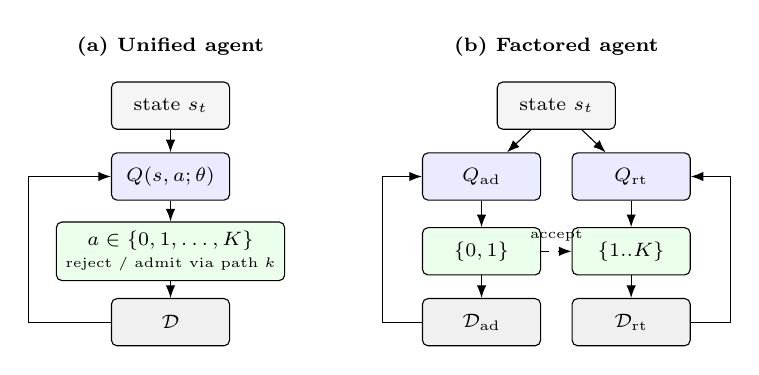
\begin{tikzpicture}[
  font=\scriptsize,
  box/.style={draw,rounded corners=2pt,minimum height=6mm,minimum width=15mm,align=center},
  net/.style={box,fill=blue!8},
  buf/.style={box,fill=black!6},
  >={Latex[length=1.6mm]}
]
% ---- unified ----
\node[align=center] at (0,1.35) {\textbf{(a) Unified agent}};
\node[box,fill=black!4] (s1) at (0,0.6) {state $s_t$};
\node[net] (q1) at (0,-0.3) {$Q(s,a;\theta)$};
\node[box,fill=green!8,minimum width=26mm] (a1) at (0,-1.25) {$a\in\{0,1,\dots,K\}$\\ \tiny reject / admit via path $k$};
\node[buf] (d1) at (0,-2.15) {$\mathcal{D}$};
\draw[->] (s1)--(q1); \draw[->] (q1)--(a1); \draw[->] (a1)--(d1);
\draw[->] (d1.west) -- ++(-1.05,0) |- (q1.west);
% ---- factored ----
\begin{scope}[xshift=4.9cm]
\node[align=center] at (0,1.35) {\textbf{(b) Factored agent}};
\node[box,fill=black!4] (s2) at (0,0.6) {state $s_t$};
\node[net] (qa) at (-0.95,-0.3) {$Q_{\text{ad}}$};
\node[net] (qr) at (0.95,-0.3) {$Q_{\text{rt}}$};
\node[box,fill=green!8] (aa) at (-0.95,-1.25) {$\{0,1\}$};
\node[box,fill=green!8] (ar) at (0.95,-1.25) {$\{1..K\}$};
\node[buf] (da) at (-0.95,-2.15) {$\mathcal{D}_{\text{ad}}$};
\node[buf] (dr) at (0.95,-2.15) {$\mathcal{D}_{\text{rt}}$};
\draw[->] (s2)--(qa); \draw[->] (s2)--(qr);
\draw[->] (qa)--(aa); \draw[->] (qr)--(ar);
\draw[->] (aa)--(da); \draw[->] (ar)--(dr);
\draw[->,dashed] (aa.east) -- node[above,font=\tiny]{accept} (ar.west);
\draw[->] (da.west) -- ++(-0.5,0) |- (qa.west);
\draw[->] (dr.east) -- ++(0.5,0) |- (qr.east);
\end{scope}
\end{tikzpicture}
\caption{Agent architectures. The unified agent (a) couples admission and
routing in one action space of size $K+1$ served by a single network and
replay buffer. The factored agent (b) uses independent admission and
routing estimators; the routing network is queried only when the
admission decision is to accept, and is trained from a dedicated buffer
$\mathcal{D}_{\text{rt}}$ that receives admitted transitions only.}
\label{fig:arch}
\end{figure}

\subsection{Value Decomposition and Learning Rule}
%-----------------------------------------------------------------------
% [A-P2] GUIDANCE: Give the duelling decomposition and the double-DQN
% target. Keep it brief -- these are standard -- but do state the two
% implementation choices that mattered in practice: Huber loss and
% gradient-norm clipping, and target sync every C environment STEPS
% (not episodes). Mention that all agents and the AC-only baseline share
% these, so comparisons isolate architecture rather than training
% stability.
%-----------------------------------------------------------------------
Each network decomposes its output into a state-value and an advantage
stream,
\begin{align}
Q(s,a;\theta,\alpha,\beta) &= V(s;\beta) \notag\\
&\quad + \Bigl( A(s,a;\alpha) - \tfrac{1}{|\mathcal{A}|}\textstyle\sum_{a'} A(s,a';\alpha) \Bigr),
\label{eq:duel}
\end{align}
and is trained on the double-DQN target
\begin{equation}
y_i = r_i + \gamma\,(1-\text{done}_i)\;
Q\bigl(s'_i,\; \arg\max_{a'} Q(s'_i,a';\theta);\; \theta^{-}\bigr),
\label{eq:target}
\end{equation}
minimising the Huber loss
\begin{equation}
L(\theta) = \mathbb{E}_{B\sim\mathcal{D}}
\left[ \frac{1}{|B|}\sum_{i\in B} \mathcal{L}_{\delta}\bigl(y_i - Q(s_i,a_i;\theta)\bigr) \right].
\label{eq:loss}
\end{equation}
Gradient norms are clipped and target parameters are synchronised every
$C$ environment steps. The same loss, clipping and synchronisation
schedule are used by every learned agent, including the admission-only
baseline, so that comparisons reflect architecture rather than
differences in training stability.

\subsection{Factored Agent and the Routing Buffer}
%-----------------------------------------------------------------------
% [A-P3] GUIDANCE: This is the implementation detail that makes the
% factored agent correct, and it is worth a paragraph. The routing
% network must be trained ONLY on transitions where a slice was actually
% admitted, because a rejection carries no information about which path
% would have been good. Hence two buffers: D_ad receives every
% transition, D_rt receives admitted transitions only. Note this also
% means the routing network sees a smaller but cleaner sample.
%-----------------------------------------------------------------------
In the factored agent the two estimators are trained from different
experience streams. The admission network learns from every transition,
since accepting and rejecting are both informative about the admission
decision. The routing network, however, must learn only from transitions
in which a slice was actually admitted: a rejected request exercises no
path, and its outcome carries no evidence about which path would have
been preferable. The agent therefore maintains two buffers,
$\mathcal{D}_{\text{ad}}$ receiving all transitions and
$\mathcal{D}_{\text{rt}}$ receiving admitted transitions only. The
routing network consequently trains on a smaller but uncontaminated
sample, which is the structural reason for the stability reported in
Section~\ref{sec:scaling}. Algorithm~\ref{alg:training} states the
training procedure for both architectures; the branches marked
\texttt{unified} and \texttt{factored} differ only in how experience is
stored and how many estimators are updated.

\begin{algorithm}[t]
\caption{Training loop for both agent architectures}
\label{alg:training}
\scriptsize
\begin{algorithmic}[1]
\State \textbf{Input:} topology $G(V,E)$, episodes $M$, steps per episode $T$
\If{\texttt{unified}}
    \State initialise $Q(\cdot;\theta)$, target $\hat{Q}(\cdot;\theta^-)$, buffer $\mathcal{D}$
\Else
    \State initialise $Q_{\text{ad}}(\cdot;\theta_{\text{ad}})$, $Q_{\text{rt}}(\cdot;\theta_{\text{rt}})$ and targets
    \State initialise buffers $\mathcal{D}_{\text{ad}}$, $\mathcal{D}_{\text{rt}}$
\EndIf
\State $n \gets 0$ \Comment{global step counter}
\For{episode $=1$ to $M$}
  \State reset environment, observe $s_0$
  \For{$t=1$ to $T$}
    \State compute $\boldsymbol{\phi}$ from $\mathbf{B}$, $\mathbf{M}_t$, $b_t$ \Comment{Eq.~\eqref{eq:phi}}
    \If{\texttt{unified}}
        \State $a_t \gets \epsilon\text{-greedy}\bigl(Q(s_t,\cdot;\theta)\bigr)$
    \Else
        \State $a^{\text{ad}} \gets \epsilon\text{-greedy}\bigl(Q_{\text{ad}}(s_t,\cdot)\bigr)$
        \If{$a^{\text{ad}} = 1$}
            \State $a^{\text{rt}} \gets \epsilon\text{-greedy}\bigl(Q_{\text{rt}}(s_t,\cdot)\bigr)$
        \Else
            \State $a^{\text{rt}} \gets \varnothing$
        \EndIf
    \EndIf
    \State execute action (Algorithm~\ref{alg:step}), observe $r_t$, $s_{t+1}$
    \If{\texttt{unified}}
        \State push $(s_t,a_t,r_t,s_{t+1})$ to $\mathcal{D}$
    \Else
        \State push $(s_t,a^{\text{ad}},r_t,s_{t+1})$ to $\mathcal{D}_{\text{ad}}$
        \If{$a^{\text{ad}} = 1$} push $(s_t,a^{\text{rt}},r_t,s_{t+1})$ to $\mathcal{D}_{\text{rt}}$
        \EndIf
    \EndIf
    \State sample mini-batch(es), form targets by~\eqref{eq:target}, minimise~\eqref{eq:loss}
    \State $n \gets n+1$
    \If{$n \bmod C = 0$} synchronise target parameters \EndIf
  \EndFor
\EndFor
\State \textbf{return} trained network(s)
\end{algorithmic}
\end{algorithm}

\begin{algorithm}[t]
\caption{Environment step: admission and reservation}
\label{alg:step}
\scriptsize
\begin{algorithmic}[1]
\State \textbf{Input:} request $r_t$, action (reject, or admit via path $k$)
\If{action is reject}
   \State \textbf{return} reward $0$
\EndIf
\State $\mathcal{C} \gets \{(i,j) : \mathbf{M}_t(i,j)=1\}$
\ForAll{$(i,j) \in \mathcal{C}$}
   \State $P_{i,j} \gets k$-th path of $\mathcal{P}_{i,j}$
   \If{$P_{i,j}$ undefined \textbf{or} $\min_{e \in P_{i,j}} A_e < b_t$}
       \State \textbf{return} reward $0$ \Comment{attempt fails; nothing reserved}
   \EndIf
\EndFor
\ForAll{$(i,j) \in \mathcal{C}$} \Comment{all connections verified first}
   \State $A_e \gets A_e - b_t \quad \forall e \in P_{i,j}$
\EndFor
\State register slice with lifetime $d_t$
\State \textbf{return} reward $1$
\State \textbf{on expiry:} $A_e \gets A_e + b_t$ for every reserved link
\end{algorithmic}
\end{algorithm}

%-----------------------------------------------------------------------
% [A-P4] GUIDANCE: One paragraph explaining Algorithm 2, in particular
% the two-pass structure: ALL required connections are verified before
% ANY capacity is reserved, so a slice is never partially embedded. This
% is what guarantees the fulfilment ratio of 1 claimed in Sec III-B.
%-----------------------------------------------------------------------
Algorithm~\ref{alg:step} details the environment transition. Its two-pass
structure matters: every required logical connection is verified against
the residual capacity before any reservation is made, so a slice is never
partially embedded. Together with the release of capacity on expiry, this
is what guarantees that every admitted slice is served at its requested
rate throughout its lifetime.

%=======================================================================
\section{Simulation Framework and Experimental Protocol} \label{expSetup}
%=======================================================================

\subsection{Framework}
%-----------------------------------------------------------------------
% [E-P1] GUIDANCE: Describe the framework honestly. It is a flow-level
% discrete-event simulator implementing the Gymnasium API, with agents in
% PyTorch, packaged in Docker for reproducible GPU execution. An Open
% vSwitch interface exists for data-plane instantiation of the computed
% embeddings. BE PRECISE: the results reported in this paper come from
% the flow-level simulator; the OVS path is used for feasibility
% validation of the produced configurations, not to produce the numbers.
% Do NOT claim packet-level measurements -- we did not make any.
%-----------------------------------------------------------------------
Experiments are run in a flow-level discrete-event simulator implementing
the Gymnasium API, with agents implemented in PyTorch and the whole stack
containerised so that runs are reproducible on GPU servers. One
simulation step corresponds to one slice arrival event; slice lifetimes
are decremented every step and reserved capacity is returned on expiry.
An Open vSwitch interface allows the embeddings produced by a trained
policy to be instantiated on an emulated data plane, which we use to
verify that the computed reservations correspond to realisable
forwarding state. All performance figures reported in this paper are
obtained from the flow-level simulator.

\subsection{Topologies}
%-----------------------------------------------------------------------
% [E-P2] GUIDANCE: Describe both topologies and, crucially, WHY there are
% two: to separate results that generalise from results that are
% artefacts of one graph. Give the numbers from
% Table~\ref{tab:topologies}. Emphasise that the second topology is
% deliberately dissimilar (different size, different generative model,
% heterogeneous capacities) and that the capacity scale was chosen so
% that the greedy baseline operates at a comparable acceptance level
% (~0.47) -- this isolates topology as the variable rather than load.
%-----------------------------------------------------------------------
Two substrates are used. The first is a real operator topology with $86$
nodes, of which $21$ are slice endpoints and the remainder provide
transit. The second is deliberately dissimilar: a synthetic graph whose
core is generated by the Waxman random-geometric model, with fewer
endpoints, a different degree distribution and heterogeneous link
capacities. Using two substrates lets us separate conclusions that
generalise from those that are properties of a single graph. Their
characteristics are given in Table~\ref{tab:topologies}. The capacity
scale of the second topology was set so that the greedy baseline operates
at a comparable acceptance level, isolating topology rather than offered
load as the variable under study.

\begin{table}[t]
\centering
\caption{Characteristics of the two evaluation substrates.}
\label{tab:topologies}
\renewcommand{\arraystretch}{1.15}
\begin{tabular}{lcc}
\toprule
& \textbf{Operator} & \textbf{Waxman} \\
\midrule
Total nodes                       & $86$    & $39$ \\
Endpoint nodes $|V_a|$            & $21$    & $15$ \\
Links                             & $106$   & $71$ \\
Link capacity                     & uniform & heterogeneous \\
Endpoint pairs with $\geq 3$ paths & $96.7\%$ & $100\%$ \\
State dimension \eqref{eq:statedim} ($K{=}3$) & $1773$ & $909$ \\
Greedy acceptance at operating point & $0.4637$ & $0.4665$ \\
Routing headroom $\rho$ \eqref{eq:rho} & $\mathbf{11.0\%}$ & $\mathbf{0.0\%}$ \\
\bottomrule
\end{tabular}
\end{table}

%-----------------------------------------------------------------------
% [E-P3] GUIDANCE: Highlight the last row of the table -- it is the key
% experimental lever of the paper. The two substrates happen to differ
% almost maximally in rho (11.0% vs 0.0%) while being matched in greedy
% acceptance. State that this makes them a natural controlled test of the
% hypothesis from Sec III-E: same difficulty for admission, opposite
% conditions for routing.
%-----------------------------------------------------------------------
The final two rows of Table~\ref{tab:topologies} are what makes this pair
useful. The two substrates are matched in the difficulty they present to
an admission controller, both admitting roughly $47\%$ of arrivals under
the greedy policy, yet they differ almost maximally in routing headroom:
on the operator topology $11.0\%$ of arrivals are admissible only on a
non-shortest path, whereas on the Waxman topology the shortest path is
sufficient whenever any path is. They therefore constitute a controlled
test of the hypothesis of Section~\ref{model}.

\subsection{Traffic Model, Baselines and Metrics}
%-----------------------------------------------------------------------
% [E-P4] GUIDANCE: Traffic model in one short paragraph (Poisson
% arrivals, geometric lifetimes, uniform bandwidth, 1-3 logical
% connections per request, equal split inelastic/elastic), pointing at
% Table~\ref{tab:hyper} for values.
%-----------------------------------------------------------------------
Slice requests arrive as a Poisson process. Lifetimes are geometrically
distributed, bandwidth demands are drawn uniformly, and each request
requires between one and three logical connections between randomly
selected endpoints, with inelastic and elastic types equally likely.
Parameter values are listed in Table~\ref{tab:hyper}.

%-----------------------------------------------------------------------
% [E-P5] GUIDANCE: The baselines. Describe all three and be explicit that
% greedy is a STRONG baseline, not a straw man: it admits every feasible
% request and selects the path with the largest bottleneck, i.e. it is
% both capacity-aware and routing-aware, and it never makes a routing
% error. Saying this protects you from the reviewer suspicion that the
% DRL gains come from a weak comparator -- and it makes the modest margin
% credible rather than disappointing.
%-----------------------------------------------------------------------
Three baselines are used. \emph{Greedy} admits every request for which at
least one candidate path is feasible and routes it over the path with the
largest residual bottleneck. It is deliberately strong: it is
capacity-aware, it is routing-aware, it never rejects a request it could
serve, and by construction it never selects an infeasible path. It is
therefore optimal among memoryless policies, and any improvement over it
must come from foresight rather than from better instantaneous decisions.
\emph{Revenue threshold} admits a request only when $d_t p_t$ exceeds a
calibrated threshold and routes it over the shortest path. \emph{AC-only
DQN} learns the admission decision with the same network, loss and
training schedule as the joint agents, but always routes over the
shortest path; it isolates the contribution of learning the routing
decision.

%-----------------------------------------------------------------------
% [E-P6] GUIDANCE: Metrics and statistical protocol -- state this
% carefully, it is what makes the small margins defensible.
%   - acceptance ratio is the metric (fulfilment is identically 1, Sec III-B).
%   - 5 training seeds (42-46) for the main table, 3 for secondary studies.
%   - every agent evaluated on HELD-OUT traffic (seed+100), 200 episodes,
%     epsilon = 0, i.e. ~100k arrivals per evaluation.
%   - all agents within a seed see the SAME traffic, so comparisons are
%     PAIRED; we report paired t-tests over seeds. Explain why pairing
%     matters: it removes traffic variance and is far more powerful than
%     comparing independent means at n=5.
%-----------------------------------------------------------------------
The reported metric is the acceptance ratio, the fraction of arriving
requests that are admitted; as established in Section~\ref{model} the
fulfilment ratio is identically one under hard capacity enforcement. Each
configuration is trained with five independent seeds for the principal
comparison and three for the secondary studies. Every trained policy is
then evaluated with exploration disabled on held-out traffic generated
from a seed disjoint from training, for $200$ episodes, approximately
$10^5$ arrivals per evaluation. Within a seed all policies are evaluated
on identical traffic, so comparisons are paired and we report paired
$t$-tests across seeds. Pairing removes the between-seed traffic variance
and is substantially more powerful than comparing independent means at
this sample size, which matters because the effects we report are small.

\begin{table}[t]
\centering
\caption{Environment and training parameters.}
\label{tab:hyper}
\renewcommand{\arraystretch}{1.15}
\begin{tabular}{lc}
\toprule
\textbf{Parameter} & \textbf{Value} \\
\midrule
Candidate paths $K$              & $3$ (also $6$, $8$) \\
Arrival rate $\lambda$           & $5.0$ \\
Mean slice lifetime              & $30$ \\
Bandwidth demand                 & $\mathcal{U}[10,100]$ Mb/s \\
Logical connections per request  & $\mathcal{U}\{1,2,3\}$ \\
$\Pr[\text{inelastic}]$          & $0.5$ \\
\midrule
Episodes $M$ / steps $T$         & $2000$ / $500$ \\
Discount $\gamma$                & $0.99$ \\
Learning rate                    & $10^{-4}$ \\
Hidden units                     & $256$ \\
Mini-batch size                  & $64$ \\
Replay capacity                  & $5\times10^{4}$ \\
$\epsilon$: start $\to$ end      & $1.0 \to 0.05$ \\
$\epsilon$ decay steps           & $2\times10^{5}$ \\
Target sync interval $C$ (steps) & $100$ \\
Training seeds                   & $42$--$46$ \\
Evaluation                       & held-out seed, $200$ episodes, $\epsilon=0$ \\
\bottomrule
\end{tabular}
\end{table}

%=======================================================================
\section{Results} \label{results}
%=======================================================================

\subsection{Acceptance on the Operator Topology}
\label{sec:main}
%-----------------------------------------------------------------------
% [R-P1] GUIDANCE: Present Table~\ref{tab:main} and Fig.~\ref{fig:main}.
% Numbers to quote: unified 0.4806 +- 0.0043; separated 0.4739 +- 0.0049;
% greedy 0.4637 +- 0.0028; AC-only 0.4476 +- 0.0022; revenue 0.1308.
% Paired: unified vs greedy +3.6% (t=7.44, 5/5 seeds); vs AC-only +7.4%
% (t=11.60); vs revenue +267.5%. Ordering: joint > separated > greedy >
% AC-only > revenue-threshold.
% Tone: state the result plainly, do NOT oversell 3.6%.
%-----------------------------------------------------------------------
Table~\ref{tab:main} reports acceptance on the operator topology with
$K=3$, and Fig.~\ref{fig:main} shows the same comparison graphically. The
joint unified agent admits $48.06\%$ of arrivals against $46.37\%$ for
greedy, an improvement of $3.6\%$ that is consistent across all five
seeds and significant under a paired test ($t=7.44$). The margin over the
admission-only agent is larger, $7.4\%$ ($t=11.60$), and the
revenue-threshold heuristic is far behind at $13.08\%$, since a policy
that selects requests by price alone ignores the state of the network
entirely.

%-----------------------------------------------------------------------
% [R-P2] GUIDANCE: Interpret the size of the margin honestly and
% pre-empt the obvious criticism. Argument to make: greedy is a strong,
% capacity- and routing-aware comparator that is optimal among memoryless
% policies, so a 3.6% margin is the value of foresight alone, not the
% value of "using ML instead of a heuristic". Also note the contrast with
% the revenue heuristic (+267%), and warn the reader that large reported
% gains in this literature often come from weak comparators. This
% paragraph is where you earn reviewer trust.
%-----------------------------------------------------------------------
The magnitude of this margin deserves comment. Greedy is not a naive
comparator: it never declines a request it could serve and never chooses
an infeasible path, so it is optimal among policies without memory. The
$3.6\%$ improvement is therefore attributable entirely to foresight --
to decisions whose benefit is realised only at later arrivals -- and not
to better instantaneous judgement. The contrast with the
revenue-threshold heuristic, which the same agent outperforms by more
than a factor of three, illustrates how strongly reported improvements in
this literature depend on the strength of the comparator.

\begin{table}[t]
\centering
\caption{Acceptance ratio on the operator topology ($K=3$, five seeds,
held-out evaluation). Paired statistics are computed against the unified
joint agent on identical traffic.}
\label{tab:main}
\renewcommand{\arraystretch}{1.2}
\begin{tabular}{lccc}
\toprule
\textbf{Policy} & \textbf{Acceptance} & \textbf{$\Delta$ vs.\ joint} & \textbf{Paired $t$} \\
\midrule
Joint, unified      & $\mathbf{0.4806 \pm 0.0043}$ & --- & --- \\
Joint, factored     & $0.4739 \pm 0.0049$ & $-1.4\%$ & $-2.13$ (n.s.) \\
Greedy              & $0.4637 \pm 0.0028$ & $-3.6\%$ & $7.44^{*}$ \\
AC-only DQN         & $0.4476 \pm 0.0022$ & $-7.4\%$ & $11.60^{*}$ \\
Revenue threshold   & $0.1308 \pm 0.0011$ & $-267.5\%$ & $187.11^{*}$ \\
\bottomrule
\multicolumn{4}{l}{\footnotesize $^{*}$ significant at $\alpha=0.05$ ($t_{\text{crit}}=2.776$, $\mathrm{df}=4$).}
\end{tabular}
\end{table}

\begin{figure}[t]
\centering
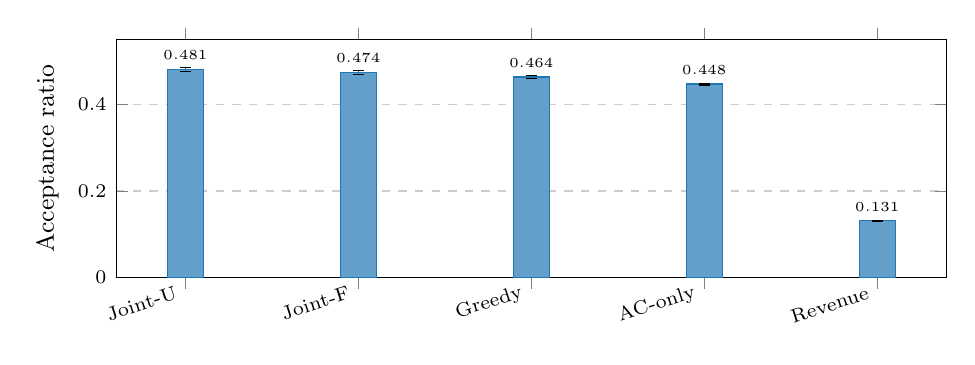
\begin{tikzpicture}
\begin{axis}[
  width=\columnwidth, height=4.6cm,
  ybar, bar width=13pt,
  ymin=0.0, ymax=0.55,
  ylabel={Acceptance ratio},
  symbolic x coords={Joint-U,Joint-F,Greedy,AC-only,Revenue},
  xtick=data, x tick label style={font=\scriptsize,rotate=18,anchor=east},
  ylabel style={font=\small}, tick label style={font=\scriptsize},
  ymajorgrids, grid style={dashed,black!20},
  error bars/y dir=both, error bars/y explicit,
  nodes near coords, every node near coord/.append style={font=\tiny,/pgf/number format/fixed,/pgf/number format/precision=3},
]
\addplot[draw=cUni,fill=cUni!70] coordinates {
  (Joint-U,0.4806) +- (0,0.0043)
  (Joint-F,0.4739) +- (0,0.0049)
  (Greedy,0.4637)  +- (0,0.0028)
  (AC-only,0.4476) +- (0,0.0022)
  (Revenue,0.1308) +- (0,0.0011)
};
\end{axis}
\end{tikzpicture}
\caption{Acceptance ratio on the operator topology ($K=3$, mean and
standard deviation over five seeds). All learned joint policies exceed
the greedy baseline; the revenue-threshold heuristic, which ignores
network state, is far behind.}
\label{fig:main}
\end{figure}

%-----------------------------------------------------------------------
% [R-P3] GUIDANCE: Learning curves, Fig.~\ref{fig:learning}. Points to
% make: both architectures converge to a similar level; the factored
% agent learns more slowly early on because its routing network only sees
% admitted transitions and therefore accumulates experience more slowly;
% both are stable, no divergence. Mention that the curves are training
% window averages and therefore sit below the held-out epsilon=0 numbers.
%-----------------------------------------------------------------------
Fig.~\ref{fig:learning} shows the training progression of both
architectures. The factored agent improves more slowly during the early
episodes, which is expected: its routing estimator only receives
transitions in which a slice was admitted, so it accumulates usable
experience at a fraction of the rate of the admission estimator. Both
architectures converge to a comparable level without instability. The
curves are averages over the training window with exploration still
active and therefore lie below the held-out values of
Table~\ref{tab:main}.

\begin{figure}[t]
\centering
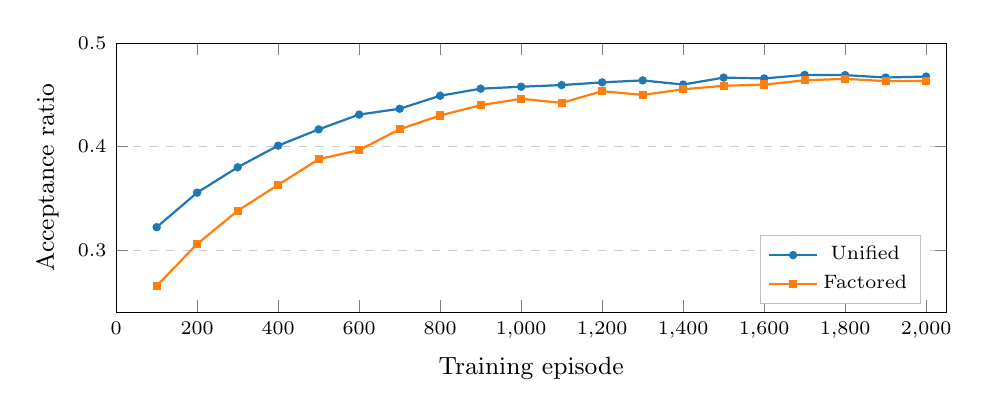
\begin{tikzpicture}
\begin{axis}[
  width=\columnwidth, height=5cm,
  xlabel={Training episode}, ylabel={Acceptance ratio},
  xlabel style={font=\small}, ylabel style={font=\small},
  tick label style={font=\scriptsize},
  xmin=0,xmax=2050, ymin=0.24, ymax=0.50,
  legend pos=south east, legend style={font=\scriptsize,draw=black!25},
  ymajorgrids, grid style={dashed,black!20},
]
\addplot[color=cUni,thick,mark=*,mark size=1.1pt] coordinates {
(100,0.3222)(200,0.3556)(300,0.3801)(400,0.4010)(500,0.4167)(600,0.4310)
(700,0.4366)(800,0.4492)(900,0.4560)(1000,0.4579)(1100,0.4595)(1200,0.4621)
(1300,0.4640)(1400,0.4600)(1500,0.4667)(1600,0.4659)(1700,0.4693)(1800,0.4691)
(1900,0.4668)(2000,0.4677)};
\addlegendentry{Unified}
\addplot[color=cSep,thick,mark=square*,mark size=1.1pt] coordinates {
(100,0.2655)(200,0.3060)(300,0.3381)(400,0.3631)(500,0.3879)(600,0.3967)
(700,0.4168)(800,0.4301)(900,0.4401)(1000,0.4462)(1100,0.4423)(1200,0.4536)
(1300,0.4500)(1400,0.4554)(1500,0.4588)(1600,0.4599)(1700,0.4641)(1800,0.4655)
(1900,0.4633)(2000,0.4634)};
\addlegendentry{Factored}
\end{axis}
\end{tikzpicture}
\caption{Training progression on the operator topology (seed $42$).
The factored agent converges more slowly because its routing estimator
is updated only from admitted transitions, but reaches a comparable
level.}
\label{fig:learning}
\end{figure}

\subsection{What the Agent Learns: Admissibility Preservation}
\label{sec:mechanism}
%-----------------------------------------------------------------------
% [R-P4] GUIDANCE: This is the most important subsection in the paper.
% Set up the question: WHY does the learned policy beat a policy that
% never refuses a feasible request? The answer must be that it declines
% some admissible requests in order to keep the substrate routable.
% Introduce the measurement: the fraction of arrivals for which at least
% one candidate path is feasible, measured ALONG EACH POLICY'S OWN
% TRAJECTORY (this is the subtle and important point -- it is an
% endogenous quantity, a consequence of the policy's own history).
%-----------------------------------------------------------------------
The greedy policy never declines a request it could serve, so an agent
that admits more requests than greedy must be creating admission
opportunities that would not otherwise exist. To identify the mechanism
we measure, along each policy's own trajectory, the fraction of arrivals
for which at least one candidate path is feasible. This quantity is
endogenous: it is determined by the capacity the policy has previously
committed, and it therefore measures the extent to which a policy has
preserved its own future freedom of action.

%-----------------------------------------------------------------------
% [R-P5] GUIDANCE: Report Table~\ref{tab:mechanism} and
% Fig.~\ref{fig:mechanism}. Numbers: operator topology, DRL keeps 54.89%
% of arrivals feasible vs greedy 46.19% (+8.7pp); Waxman 53.27% vs 46.68%
% (+6.6pp). Interpretation: by declining a minority of admissible
% requests -- typically those whose embedding would consume scarce shared
% links -- the agent keeps the substrate in a state where a larger share
% of FUTURE arrivals can be served, and ends up admitting more in total.
% This is the definition of non-myopic behaviour and it is not available
% to any memoryless heuristic.
%-----------------------------------------------------------------------
Table~\ref{tab:mechanism} reports the result and Fig.~\ref{fig:mechanism}
displays it. On the operator topology the learned policy sustains
$54.89\%$ feasible arrivals against $46.19\%$ under greedy, a difference
of $8.7$ percentage points, and the same effect appears on the Waxman
topology at $53.27\%$ against $46.68\%$. The interpretation is direct:
by declining a minority of admissible requests -- characteristically
those whose embedding would consume capacity on heavily shared links --
the agent maintains the substrate in a state in which a larger fraction
of subsequent arrivals can still be served, and admits more slices in
aggregate as a result. This is precisely the behaviour that a memoryless
policy cannot exhibit, and it is the reason the margin in
Table~\ref{tab:main} exists at all.

\begin{table}[t]
\centering
\caption{Decision decomposition and admissibility preservation
(three seeds, held-out evaluation). Feasible arrivals are measured along
each policy's own trajectory.}
\label{tab:mechanism}
\renewcommand{\arraystretch}{1.2}
\begin{tabular}{lcc}
\toprule
& \textbf{Operator} & \textbf{Waxman} \\
\midrule
Feasible arrivals, learned policy & $54.89\%$ & $53.27\%$ \\
Feasible arrivals, greedy         & $46.19\%$ & $46.68\%$ \\
\textbf{Preservation gain}        & $\mathbf{+8.70}$ pp & $\mathbf{+6.59}$ pp \\
\midrule
Admitted                          & $47.06\%$ & $48.50\%$ \\
Routing errors                    & $4.60\%$  & $0.00\%$ \\
Missed admissions                 & $3.23\%$  & $4.77\%$ \\
\bottomrule
\end{tabular}
\end{table}

\begin{figure}[t]
\centering
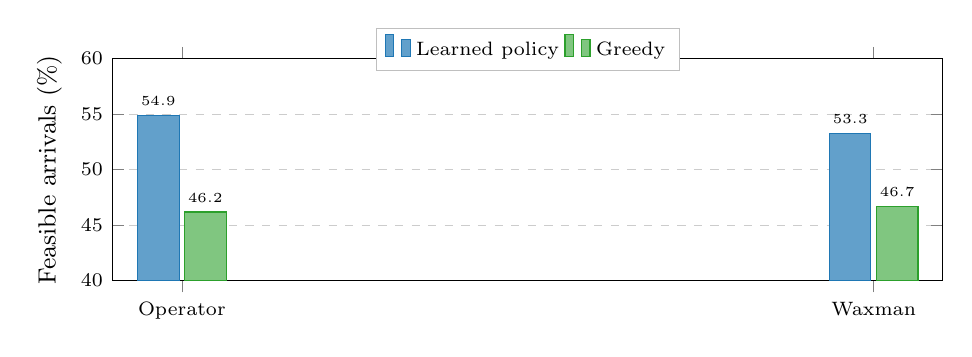
\begin{tikzpicture}
\begin{axis}[
  width=\columnwidth, height=4.4cm,
  ybar, bar width=15pt,
  ymin=40, ymax=60,
  ylabel={Feasible arrivals (\%)},
  symbolic x coords={Operator,Waxman},
  xtick=data, tick label style={font=\scriptsize}, ylabel style={font=\small},
  legend style={font=\scriptsize,at={(0.5,1.14)},anchor=north,legend columns=2,draw=black!25},
  ymajorgrids, grid style={dashed,black!20},
  nodes near coords, every node near coord/.append style={font=\tiny,/pgf/number format/fixed,/pgf/number format/precision=1},
]
\addplot[draw=cUni,fill=cUni!70] coordinates {(Operator,54.89) (Waxman,53.27)};
\addlegendentry{Learned policy}
\addplot[draw=cGre,fill=cGre!60] coordinates {(Operator,46.19) (Waxman,46.68)};
\addlegendentry{Greedy}
\end{axis}
\end{tikzpicture}
\caption{Admissibility preservation. The learned policy keeps a
substantially larger fraction of future arrivals routable than greedy on
both substrates, which is the mechanism behind its higher acceptance.}
\label{fig:mechanism}
\end{figure}

%-----------------------------------------------------------------------
% [R-P6] GUIDANCE: Use the last two rows of Table~\ref{tab:mechanism} to
% bound the headroom honestly. On the operator topology the agent still
% wastes 4.60% of arrivals on routing errors and 3.23% on missed
% admissions, i.e. ~7.8pp of its own opportunity is unexploited. Say
% plainly that the policy is not optimal and that this bounds how much
% further tuning could gain -- and forward-reference the masking
% experiment (Sec VII-F) which shows this residue is not trivially
% recoverable.
%-----------------------------------------------------------------------
The remaining rows bound how far the learned policy is from exploiting
its own advantage. On the operator topology it still attempts admission
on an infeasible path in $4.60\%$ of arrivals and declines a feasible
request in a further $3.23\%$, so close to eight percentage points of the
opportunity it creates go unused. The policy is therefore clearly
suboptimal. As Section~\ref{sec:ablations} shows, however, this residue
is not trivially recoverable: the obvious intervention of masking
infeasible actions degrades rather than improves performance.

\subsection{Generalisation and the Condition for Joint Routing}
\label{sec:generalization}
%-----------------------------------------------------------------------
% [R-P7] GUIDANCE: Open by stating what is being tested: whether the
% Sec VII-A ordering is a property of the method or of the operator
% graph. Then give the headline of Table~\ref{tab:topo2}: joint vs greedy
% REPLICATES at +3.8% (3/3 seeds, t=10.53, significant); so the core
% claim generalises.
%-----------------------------------------------------------------------
The results of Section~\ref{sec:main} were obtained on a single
substrate, and it is legitimate to ask whether they describe the method
or the graph. Table~\ref{tab:topo2} repeats the comparison on the Waxman
topology. The central result replicates: the joint agent admits $3.8\%$
more slices than greedy, on all three seeds and with a significant
paired statistic. The advantage of a learned, non-myopic admission
policy over a strong memoryless one is therefore a property of the
method rather than of the operator topology.

%-----------------------------------------------------------------------
% [R-P8] GUIDANCE: Now the finding that flips. On the Waxman topology the
% AC-only agent is the BEST policy: 0.4957 vs joint 0.4841 vs greedy
% 0.4665. AC-only beats greedy by +6.3% (t=10.04, significant) and beats
% the joint agent on all three seeds by 2.3%. BE PRECISE about
% significance: the joint-vs-AC-only difference is consistent (3/3) but
% with n=3 it does not reach the alpha=0.05 threshold (t=-3.42 vs
% t_crit=4.303). Say so explicitly. The direction is nevertheless clear
% and is corroborated by the mechanism data.
%-----------------------------------------------------------------------
One ordering does not replicate, and it is the informative one. On the
Waxman topology the admission-only agent is the strongest policy tested,
admitting $49.57\%$ of arrivals: it exceeds greedy by $6.3\%$ and
outperforms the joint agent on every seed. With three seeds this last
difference does not reach the $\alpha=0.05$ threshold in a paired test
($t=-3.42$ against $t_{\text{crit}}=4.303$), so we describe it as a
consistent direction rather than a significant effect; but its
explanation, given below, is unambiguous.

\begin{table}[t]
\centering
\caption{Acceptance ratio on the Waxman topology (three seeds, held-out
evaluation). Paired statistics against the joint unified agent.}
\label{tab:topo2}
\renewcommand{\arraystretch}{1.2}
\begin{tabular}{lccc}
\toprule
\textbf{Policy} & \textbf{Acceptance} & \textbf{$\Delta$ vs.\ joint} & \textbf{Paired $t$} \\
\midrule
AC-only DQN        & $\mathbf{0.4957 \pm 0.0055}$ & $+2.3\%$ & $-3.42$ (n.s.) \\
Joint, unified     & $0.4841 \pm 0.0021$ & --- & --- \\
Greedy             & $0.4665 \pm 0.0009$ & $-3.8\%$ & $10.53^{*}$ \\
Revenue threshold  & $0.1530$ & --- & --- \\
\bottomrule
\multicolumn{4}{l}{\footnotesize $^{*}$ significant at $\alpha=0.05$ ($t_{\text{crit}}=4.303$, $\mathrm{df}=2$).}
\end{tabular}
\end{table}

%-----------------------------------------------------------------------
% [R-P9] GUIDANCE: The explanation, tying back to rho. On the operator
% topology rho = 11.0% (23.8% of admittable arrivals need a non-shortest
% path) and the joint agent beats AC-only by 7.4%. On the Waxman topology
% rho = 0.0% EXACTLY -- the shortest path is feasible whenever any path
% is -- and the routing action space can therefore contribute nothing
% while still enlarging the space the agent must search. The measured
% routing-error rates corroborate: 4.60% on the operator topology vs
% 0.00% on Waxman. Reference Fig.~\ref{fig:rho}. This is the paper's
% boundary condition and should be stated as a practical rule.
%-----------------------------------------------------------------------
The explanation is the routing headroom of Definition~\ref{def:rho}. On
the operator topology $\rho = 11.0\%$: roughly one arrival in nine is
admissible only over a non-shortest path, and just under a quarter of all
admissible arrivals require the routing decision to be made correctly. In
that regime learning to route adds reach, and the joint agent
outperforms the admission-only agent by $7.4\%$. On the Waxman topology
$\rho = 0.0\%$ exactly; the shortest path is feasible whenever any path
is. Routing can then contribute nothing, while the enlarged action space
still has to be explored and estimated, so the joint formulation pays a
cost for a capability it cannot use. The measured routing-error rates in
Table~\ref{tab:mechanism} corroborate this reading, falling from $4.60\%$
on the operator topology to $0.00\%$ on the Waxman one.
Fig.~\ref{fig:rho} summarises the relationship.

\begin{figure}[t]
\centering
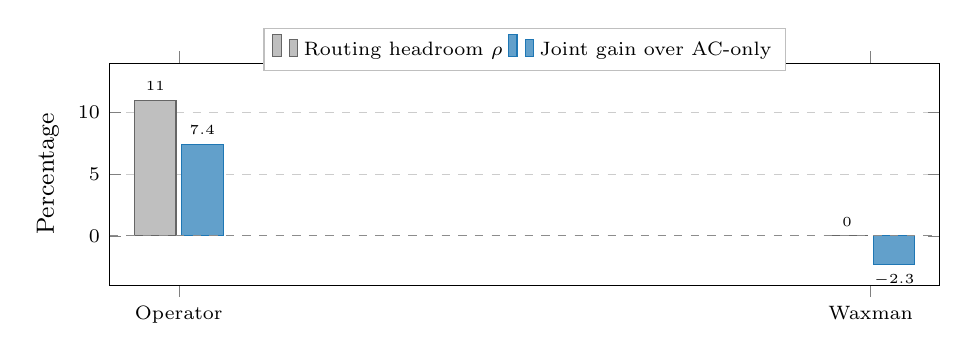
\begin{tikzpicture}
\begin{axis}[
  width=\columnwidth, height=4.4cm,
  ybar, bar width=15pt,
  ymin=-4, ymax=14,
  ylabel={Percentage},
  symbolic x coords={Operator,Waxman},
  xtick=data, tick label style={font=\scriptsize}, ylabel style={font=\small},
  legend style={font=\scriptsize,at={(0.5,1.16)},anchor=north,legend columns=2,draw=black!25},
  ymajorgrids, grid style={dashed,black!20},
  nodes near coords, every node near coord/.append style={font=\tiny,/pgf/number format/fixed,/pgf/number format/precision=1},
]
\addplot[draw=black!60,fill=black!25] coordinates {(Operator,11.0) (Waxman,0.0)};
\addlegendentry{Routing headroom $\rho$}
\addplot[draw=cUni,fill=cUni!70] coordinates {(Operator,7.4) (Waxman,-2.3)};
\addlegendentry{Joint gain over AC-only}
\draw[dashed,black!45] ({rel axis cs:0,0}|-{axis cs:Operator,0}) -- ({rel axis cs:1,0}|-{axis cs:Operator,0});
\end{axis}
\end{tikzpicture}
\caption{Routing headroom predicts the value of joint control. Where
$\rho$ is substantial the joint agent outperforms the admission-only
agent; where $\rho$ vanishes the routing action space is unusable and the
simpler agent is preferable. $\rho$ is obtained without training.}
\label{fig:rho}
\end{figure}

%-----------------------------------------------------------------------
% [R-P10] GUIDANCE: State the practical implication as a deployment rule,
% because this is what an operator would actually use. Rule: compute rho
% from the topology and the expected traffic profile; if it is close to
% zero, deploy the admission-only controller, which is smaller, trains
% faster and performs better; if it is materially positive, the joint
% controller is justified. Note the cost asymmetry: deploying joint where
% rho=0 cost about 2.3% acceptance here.
%-----------------------------------------------------------------------
This yields a deployment rule that requires no training to apply. An
operator can estimate $\rho$ from the topology and an expected traffic
profile before committing to an architecture. Where $\rho$ is close to
zero the admission-only controller is preferable on every count: it is
smaller, it trains faster, and it performed better here. Where $\rho$ is
materially positive the additional complexity of joint control is
justified. The asymmetry matters, since deploying the joint controller
where routing is useless cost $2.3\%$ of acceptance in our measurements.

\subsection{Architecture and Scaling in the Number of Paths}
\label{sec:scaling}
%-----------------------------------------------------------------------
% [R-P11] GUIDANCE: Present Table~\ref{tab:scaling} and
% Fig.~\ref{fig:scaling}. Facts: at K=3 unified 0.4806 vs factored 0.4739,
% difference NOT significant (t=-2.13) -> the architectures are
% equivalent at small K. At K=6 both flat (0.4802 / 0.4752). At K=8 the
% unified agent falls to 0.4679 while the factored one holds at 0.4727.
% The unified degradation K=3 -> K=8 is -2.6% and significant (t=-5.85);
% the factored change is -0.3% and is not. The head-to-head at K=8
% (+1.0%, 4/5 seeds) is NOT significant (t=1.19), so do not claim the
% factored agent WINS at K=8 -- claim ROBUSTNESS: one architecture
% degrades, the other does not.
%-----------------------------------------------------------------------
Table~\ref{tab:scaling} and Fig.~\ref{fig:scaling} compare the two
architectures as the number of candidate paths grows. At $K=3$ they are
statistically indistinguishable, the unified agent's nominal advantage of
$1.4\%$ falling well short of significance. Both remain flat at $K=6$.
At $K=8$ they separate: the unified agent falls to $0.4679$ while the
factored agent holds at $0.4727$. The unified degradation from $K=3$ to
$K=8$ is $2.6\%$ and is significant ($t=5.85$), whereas the factored
agent changes by $0.3\%$, which is not. We are careful about what this
supports: the head-to-head difference at $K=8$ favours the factored agent
on four of five seeds but does not itself reach significance ($t=1.19$).
The defensible claim is therefore one of robustness rather than
superiority -- as the action space grows, the unified architecture
degrades and the factored one does not.

%-----------------------------------------------------------------------
% [R-P12] GUIDANCE: Explain WHY, structurally. The unified action space
% grows with K, so the admission decision must be inferred from a value
% estimate spread across K+1 entangled actions, and the estimation
% problem for the admission decision itself gets harder as K rises. The
% factored agent's admission head stays at size 2 for every K; only the
% routing head widens, and it trains from a clean admitted-only sample.
% Practical implication: prefer the factored design when many candidate
% paths are needed.
%-----------------------------------------------------------------------
The explanation is structural. In the unified formulation the admission
decision is not represented separately: whether to admit is inferred from
a value estimate spread over $K+1$ entangled actions, so the difficulty of
the admission problem itself grows with the number of paths offered. The
factored formulation keeps the admission estimator at two outputs for
every $K$, and widens only the routing estimator, which trains from the
uncontaminated admitted-only sample described in
Section~\ref{agents}. The practical implication is that the factored
design should be preferred wherever a large candidate path set is
required, and that the choice is inconsequential when $K$ is small.

\begin{table}[t]
\centering
\caption{Acceptance ratio versus the number of candidate paths $K$
(five seeds at $K=3,8$; three seeds at $K=6$).}
\label{tab:scaling}
\renewcommand{\arraystretch}{1.2}
\begin{tabular}{lccc}
\toprule
\textbf{Architecture} & $K=3$ & $K=6$ & $K=8$ \\
\midrule
Unified   & $0.4806 \pm 0.0043$ & $0.4802 \pm 0.0048$ & $0.4679 \pm 0.0071$ \\
Factored  & $0.4739 \pm 0.0049$ & $0.4752 \pm 0.0062$ & $0.4727 \pm 0.0040$ \\
\midrule
\multicolumn{4}{l}{\footnotesize Unified change $K{=}3 \to K{=}8$: $-2.6\%$ ($t=5.85$, significant).} \\
\multicolumn{4}{l}{\footnotesize Factored change $K{=}3 \to K{=}8$: $-0.3\%$ (not significant).} \\
\bottomrule
\end{tabular}
\end{table}

\begin{figure}[t]
\centering
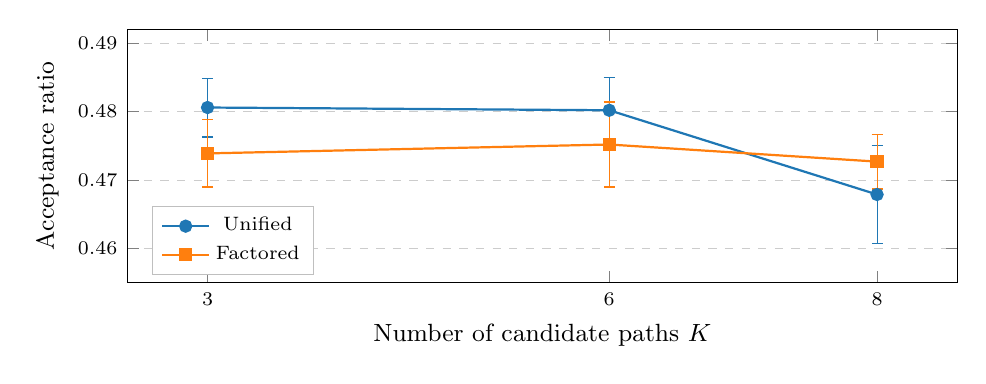
\begin{tikzpicture}
\begin{axis}[
  width=\columnwidth, height=4.8cm,
  xlabel={Number of candidate paths $K$}, ylabel={Acceptance ratio},
  xlabel style={font=\small}, ylabel style={font=\small},
  tick label style={font=\scriptsize},
  xtick={3,6,8}, xmin=2.4, xmax=8.6, ymin=0.455, ymax=0.492,
  legend pos=south west, legend style={font=\scriptsize,draw=black!25},
  ymajorgrids, grid style={dashed,black!20},
  error bars/y dir=both, error bars/y explicit,
]
\addplot[color=cUni,thick,mark=*] coordinates {
  (3,0.4806) +- (0,0.0043) (6,0.4802) +- (0,0.0048) (8,0.4679) +- (0,0.0071)};
\addlegendentry{Unified}
\addplot[color=cSep,thick,mark=square*] coordinates {
  (3,0.4739) +- (0,0.0049) (6,0.4752) +- (0,0.0062) (8,0.4727) +- (0,0.0040)};
\addlegendentry{Factored}
\end{axis}
\end{tikzpicture}
\caption{Scaling in the number of candidate paths. The unified
architecture degrades significantly between $K=3$ and $K=8$; the factored
architecture is unaffected.}
\label{fig:scaling}
\end{figure}

\subsection{Sensitivity to Offered Load}
\label{sec:load}
%-----------------------------------------------------------------------
% [R-P13] GUIDANCE: Present Table~\ref{tab:load} and
% Fig.~\ref{fig:load}. Facts: at the nominal operating point the joint
% margin over greedy is +3.6% (significant). When capacity is halved
% (acceptance drops to ~0.30) the margin falls to +1.0%, consistent on
% 3/3 seeds but NOT significant (t=2.53 vs t_crit=4.303). Meanwhile the
% margin over AC-only is preserved (+5.5%, significant).
% INTERPRETATION -- this is the interesting part: the value of foresight
% requires slack to exploit. Under severe congestion nearly every
% feasible admission is forced and there is little scope to shape the
% future, so greedy is close to optimal. The advantage of the method is
% therefore largest at moderate load, which is also the regime operators
% normally engineer for.
%-----------------------------------------------------------------------
Table~\ref{tab:load} and Fig.~\ref{fig:load} examine sensitivity to
offered load. Halving the available capacity reduces acceptance for all
policies to roughly $0.30$, and the joint agent's margin over greedy
falls from $3.6\%$ to $1.0\%$; the direction is consistent across seeds
but the difference is no longer significant at this sample size. The
margin over the admission-only agent is preserved at $5.5\%$. The
interpretation follows from the mechanism of
Section~\ref{sec:mechanism}: foresight requires slack in order to be
exercised. When capacity is severely constrained almost every feasible
admission is effectively forced and there is little room to shape which
requests remain servable later, so greedy approaches optimality. The
method is consequently most valuable at moderate utilisation -- which is
also the regime in which transport networks are normally engineered to
operate.

\begin{table}[t]
\centering
\caption{Effect of offered load on the operator topology (three seeds at
the high-load point). Capacity scale $1.0$ is the nominal operating point.}
\label{tab:load}
\renewcommand{\arraystretch}{1.2}
\begin{tabular}{lcc}
\toprule
& \textbf{Nominal} & \textbf{High load} \\
\midrule
Joint, unified      & $0.4806$ & $0.3036 \pm 0.0013$ \\
Greedy              & $0.4637$ & $0.3006 \pm 0.0026$ \\
AC-only DQN         & $0.4476$ & $0.2878 \pm 0.0025$ \\
\midrule
Joint $-$ greedy    & $+3.6\%^{*}$ & $+1.0\%$ (n.s.) \\
Joint $-$ AC-only   & $+7.4\%^{*}$ & $+5.5\%^{*}$ \\
\bottomrule
\multicolumn{3}{l}{\footnotesize $^{*}$ significant at $\alpha=0.05$.}
\end{tabular}
\end{table}

\begin{figure}[t]
\centering
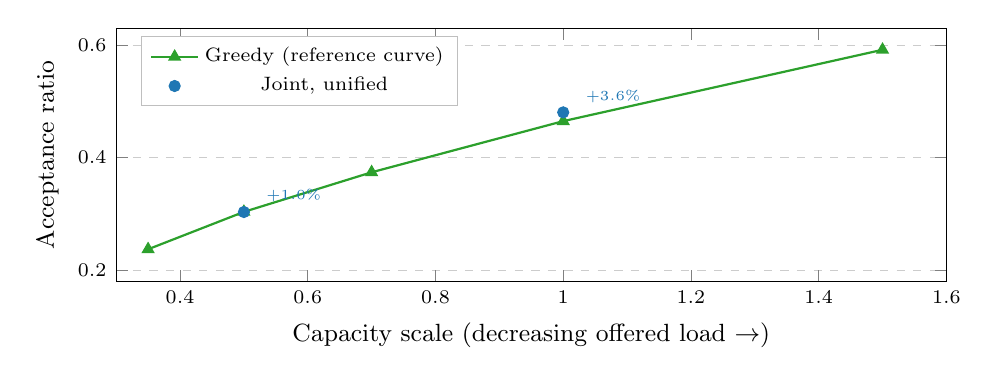
\begin{tikzpicture}
\begin{axis}[
  width=\columnwidth, height=4.8cm,
  xlabel={Capacity scale (decreasing offered load $\rightarrow$)},
  ylabel={Acceptance ratio},
  xlabel style={font=\small}, ylabel style={font=\small},
  tick label style={font=\scriptsize},
  xmin=0.3, xmax=1.6, ymin=0.18, ymax=0.63,
  legend pos=north west, legend style={font=\scriptsize,draw=black!25},
  ymajorgrids, grid style={dashed,black!20},
]
\addplot[color=cGre,thick,mark=triangle*] coordinates {
  (0.35,0.2375)(0.5,0.3039)(0.7,0.3742)(1.0,0.4650)(1.5,0.5917)};
\addlegendentry{Greedy (reference curve)}
\addplot[color=cUni,only marks,mark=*,mark size=2pt] coordinates {
  (0.5,0.3036)(1.0,0.4806)};
\addlegendentry{Joint, unified}
\node[font=\tiny,anchor=south west,cUni] at (axis cs:1.02,0.4806) {$+3.6\%$};
\node[font=\tiny,anchor=south west,cUni] at (axis cs:0.52,0.3036) {$+1.0\%$};
\end{axis}
\end{tikzpicture}
\caption{Acceptance against offered load. The greedy curve traces the
operating envelope of the substrate; the joint agent's advantage is
largest at moderate load and contracts under severe congestion, where
almost every feasible admission is forced.}
\label{fig:load}
\end{figure}

\subsection{Ablations and Negative Results}
\label{sec:ablations}
%-----------------------------------------------------------------------
% [R-P14] GUIDANCE: Action masking. Motivation: Sec VII-B showed 4.6% of
% arrivals lost to routing errors; masking infeasible paths using phi
% should recover them, and masking is standard practice
% (cite huang2022invalid). Result: it did NOT. Masked 0.4602 +- 0.0208 vs
% unmasked 0.4806 +- 0.0043 -- mean drops 4.2% and, more tellingly, the
% standard deviation grows FIVEFOLD. Be precise: because variance
% explodes, the mean difference is not itself significant (t=-2.09); the
% robust observation is the loss of stability. Offer the likely cause:
% the policy acts under the mask but the bootstrap target still maximises
% over unmasked actions, so behaviour and target policy are inconsistent.
% Note this is a property of our implementation, not proof that masking
% cannot work -- intellectual honesty here is a strength.
%-----------------------------------------------------------------------
Section~\ref{sec:mechanism} showed that $4.60\%$ of arrivals are lost to
routing errors, and the standard remedy is to mask invalid
actions~\cite{huang2022invalid}: the feasibility signal $\boldsymbol{\phi}$
identifies exactly which paths cannot serve the request, so those actions
can be removed from consideration. This did not work. With masking
enabled, acceptance fell to $0.4602 \pm 0.0208$ from $0.4806 \pm 0.0043$,
and the more informative change is in the second moment -- the standard
deviation across seeds grew roughly fivefold, with two of five runs
converging to visibly poorer policies. Because of that variance the
difference in means is not itself significant ($t=-2.09$); the robust
finding is the loss of stability rather than the loss of accuracy. The
likely cause is an inconsistency we did not correct: the behaviour policy
selects among masked actions while the bootstrap target
in~\eqref{eq:target} still maximises over the unmasked action set, so the
agent learns towards a policy it never executes. We report this as a
negative result for our implementation rather than as evidence that
masking is inapplicable to this problem.

%-----------------------------------------------------------------------
% [R-P15] GUIDANCE: The revenue-objective ablation, which justifies the
% modelling choice made in Sec III-B. Facts to state: with a revenue
% objective and soft capacity (over-admission permitted, SLA violations
% penalised) the agent DID beat greedy on discounted revenue
% (222,239 vs 219,365 per episode) -- but it did so by admitting FEWER
% slices than greedy in every regime tested. It wins the objective it is
% given, and that objective is not the one the slicing literature
% reports. This is why the count objective is used throughout.
%-----------------------------------------------------------------------
We also examined the alternative revenue objective under a soft capacity
model in which over-admission is permitted and service-level violations
are penalised. Under that formulation the learned policy did outperform
greedy on the quantity it was asked to maximise, accruing $222{,}239$
against $219{,}365$ units of net revenue per episode. It achieved this,
however, by admitting fewer slices than greedy in every regime we
examined: the agent learned to prefer expensive requests and to decline
inexpensive ones whose later violation would cost more than they earn.
The policy is correct for its objective, but that objective is not the
one under which slicing systems are conventionally assessed. This
observation motivated the count objective adopted
in~\eqref{eq:objective}.

%=======================================================================
\section{Discussion} \label{discussion}
%=======================================================================
%-----------------------------------------------------------------------
% [D-P1] GUIDANCE: Summarise which findings are robust and which are
% conditional -- this framing is the paper's main intellectual product.
% ROBUST (both topologies, both load regimes): learned non-myopic
% admission beats strong greedy; the mechanism is admissibility
% preservation. CONDITIONAL: the value of joint routing, governed by rho;
% the choice of architecture, governed by K; the size of the margin,
% governed by load.
%-----------------------------------------------------------------------
It is worth separating what these experiments establish from what they
qualify. Two findings are robust across both substrates and both load
regimes: a learned admission policy outperforms a strong memoryless
heuristic, and it does so by preserving the admissibility of future
arrivals rather than by making better instantaneous decisions. Three
further findings are conditional, and we were able to identify the
quantity governing each: the value of learning routing jointly is
governed by the routing headroom $\rho$, the choice between unified and
factored architectures is governed by the size of the candidate path
set, and the magnitude of the advantage is governed by offered load.

%-----------------------------------------------------------------------
% [D-P2] GUIDANCE: Operator-facing implications. Three concrete ones:
%   (i) measure rho first; it decides the architecture and costs nothing;
%   (ii) prefer the factored design when K is large, either is fine when
%        K is small;
%   (iii) expect the benefit at moderate utilisation, not at saturation --
%        so this is a capacity-planning aid, not a congestion remedy.
%-----------------------------------------------------------------------
For an operator considering deployment, three implications follow.
First, the routing headroom of the intended substrate and traffic mix
should be measured before an architecture is chosen, since it is
inexpensive to compute and determines whether the routing component is
worth learning at all. Second, when a large candidate path set is
required the factored architecture should be preferred, while for small
path sets the two designs are interchangeable. Third, the benefit should
be expected at moderate utilisation rather than at saturation; the method
is an aid to serving more slices from an adequately provisioned network,
not a remedy for one that is congested.

%-----------------------------------------------------------------------
% [D-P3] GUIDANCE: Threats to validity -- state them plainly, reviewers
% respect this. (i) two topologies is better than one but still not a
% population; rho is validated at only two points (11.0% and 0.0%) and
% intermediate values are untested. (ii) secondary studies use 3 seeds,
% which limits power -- we flagged every non-significant comparison.
% (iii) flow-level simulation: no packet dynamics, no queueing or
% transient effects. (iv) traffic is synthetic and stationary; real slice
% arrivals are non-stationary and correlated. (v) only value-based
% agents were studied.
%-----------------------------------------------------------------------
Several limitations qualify these conclusions. Two substrates are better
than one but do not constitute a sample; in particular $\rho$ has been
validated only at its extremes, $11.0\%$ and $0\%$, and its predictive
value at intermediate levels is untested. The secondary studies use three
seeds, which limits statistical power, and we have marked every
comparison that does not reach significance. The evaluation is at flow
level and therefore excludes queueing dynamics, transient congestion and
packet-level effects. The arrival process is synthetic and stationary,
whereas real slice demand is correlated and non-stationary. Finally, only
value-based agents were examined; policy-gradient methods may behave
differently, particularly with respect to the action masking result.

%-----------------------------------------------------------------------
% [D-P4] GUIDANCE: Future work, short and specific -- (a) sweep rho
% across a family of synthetic topologies to turn the boundary condition
% into a calibrated curve; (b) fix the masking target inconsistency;
% (c) non-stationary demand and transfer between substrates, connecting
% to wang2024flagvne.
%-----------------------------------------------------------------------
Three extensions follow naturally. Sweeping $\rho$ across a family of
synthetic substrates would convert the boundary condition from a
two-point observation into a calibrated relationship. Correcting the
target inconsistency in the masked formulation would establish whether
the residual routing errors are recoverable. Finally, evaluating transfer
across substrates and under non-stationary demand connects this work to
the generalisation agenda pursued in recent embedding
literature~\cite{wang2024flagvne}.

%=======================================================================
\section{Conclusion} \label{conclusion}
%=======================================================================
%-----------------------------------------------------------------------
% [C-P1] GUIDANCE: One paragraph restating the problem and what was
% built. One paragraph with the results in the honest order: mechanism
% first (+8.7pp / +6.6pp preservation), then the margins (+3.6% / +3.8%
% over greedy), then the boundary condition (rho: 11.0% -> joint wins by
% 7.4%; 0% -> AC-only better), then the architecture/scaling result.
% Close with the general lesson: in this problem the durable contribution
% of learning is admission foresight, and the value of adding routing is
% a measurable property of the substrate rather than a universal gain.
% Do NOT close with an inflated claim.
%-----------------------------------------------------------------------
We formulated joint slice admission control and path-level resource
allocation for an operator IP core as a Markov Decision Process whose
state uses only counters available from production telemetry, and solved
it with duelling deep Q-networks in two architectural variants.

The learned policies improve on a strong bottleneck-aware greedy
controller by $3.6\%$ on a real operator topology and by $3.8\%$ on a
structurally different synthetic one. The improvement is explained by a
single measurable behaviour: the agents preserve the admissibility of
future arrivals, sustaining $8.7$ and $6.6$ additional percentage points
of routable arrivals respectively. The value of learning routing jointly
with admission proved conditional, and we identified the substrate
statistic that governs it: where $11.0\%$ of arrivals required a
non-shortest path the joint agent outperformed an admission-only
controller by $7.4\%$, whereas on a substrate where the shortest path
always sufficed the admission-only controller was the better design.
Finally, a factored architecture with independent admission and routing
estimators matched the unified one for small path sets and remained
stable at eight candidate paths, where the unified agent lost $2.6\%$.

The broader lesson is that in this problem the durable contribution of
learning is admission foresight, while the benefit of adding routing to
the learned decision is a property of the substrate that can, and should,
be measured before the additional complexity is adopted.

\section*{Acknowledgments}
%-----------------------------------------------------------------------
% GUIDANCE: funding, institutional support, compute resources.
%-----------------------------------------------------------------------
This should be a simple paragraph before the references to thank those
individuals and institutions who supported this work.

\bibliographystyle{IEEEtran}
\bibliography{IEEEabrv,Slicing}

\begin{IEEEbiography}[{\includegraphics[width=1in,height=1.25in,clip,keepaspectratio]{./Figures/Amaral_3x4.jpg}}]
{Pedro Amaral} received the Ph.D.\ in Electrical and Computer Engineering in 2013 and the M.Sc.\ in Computer Engineering in 2006 from Universidade Nova de Lisboa. He is an Assistant Professor at Faculdade de Ci\^encias e Tecnologia, Universidade Nova de Lisboa, a researcher at Instituto de Telecomunica\c{c}\~oes, Lisboa, and an IEEE member. His research interests include model-free resource optimisation algorithms in networks, AI-enhanced network management and control, and network security.
\end{IEEEbiography}

\end{document}

%=======================================================================
%  CLAIMS AUDIT -- READ BEFORE SUBMISSION
%=======================================================================
%  Claims REMOVED from the previous version because the experiments do
%  not support them:
%
%  1. "DRL agents increase accepted and fulfilled slices by 47.5% versus
%     baseline methods."
%     -> Measured margin over the GREEDY baseline is +3.6% (operator) and
%        +3.8% (Waxman). A figure of this magnitude appears only against
%        the revenue-threshold heuristic (+267%), which is a weak
%        comparator. Reporting +47.5% without naming that comparator
%        would be misleading.
%
%  2. "Jointly solving admission control and resource allocation gives an
%     18% improvement over solving admission control alone."
%     -> Measured at +7.4% on the operator topology. Moreover the sign
%        REVERSES on the second topology (AC-only is better by 2.3%),
%        which is why the paper now presents this as conditional on rho
%        rather than as a universal result. This reversal is a finding,
%        not a failure -- it is what makes the rho contribution possible.
%
%  3. "Fulfilled slices (slices that have the desired bandwidth and
%     packet loss values)."
%     -> The current model enforces capacity strictly, so fulfilment is
%        identically 1 and carries no information. There is NO packet
%        loss model in the evaluation. Any statement about packet loss
%        must be removed or supported by new experiments.
%
%  4. The claim that agents are trained "in realistic networking
%     environments" using Open vSwitch.
%     -> All numbers reported here come from the flow-level simulator.
%        The OVS/Docker path exists but was not used to produce these
%        results. Section~\ref{expSetup} states this accurately; please
%        keep it that way.
%
%  Comparisons that are DIRECTIONAL but NOT statistically significant --
%  each is already hedged in the text; do not upgrade the language:
%     - factored vs unified at K=3   (t=-2.13, n=5)
%     - factored vs unified at K=8   (t=+1.19, n=5)
%     - joint vs AC-only on Waxman   (t=-3.42, n=3)
%     - joint vs greedy at high load (t=+2.53, n=3)
%     - masked vs unmasked           (t=-2.09, n=5)
%
%  Numbers that ARE significant and may be stated firmly:
%     - joint vs greedy, operator, K=3      +3.6%  (t=7.44,  n=5)
%     - joint vs AC-only, operator, K=3     +7.4%  (t=11.60, n=5)
%     - joint vs greedy, Waxman             +3.8%  (t=10.53, n=3)
%     - AC-only vs greedy, Waxman           +6.3%  (t=10.04, n=3)
%     - unified degradation K=3 -> K=8      -2.6%  (t=5.85,  n=5)
%     - joint vs AC-only at high load       +5.5%  (t=15.47, n=3)
%=======================================================================
